\documentclass[a4paper]{book}

\usepackage[T1]{fontenc}
\usepackage[utf8]{inputenc}
\usepackage{booktabs}
\usepackage{multicol}
\usepackage{hyperref}
\usepackage{amsmath}
\usepackage{listings}
\usepackage{graphicx}
\usepackage{textcomp}
\usepackage{gensymb}
\usepackage{xcolor}
\usepackage[labelformat=empty]{caption}

\usepackage{refcheck}
\usepackage[backend=bibtex,style=authoryear,natbib]{biblatex}
\bibliography{biblio} 

\graphicspath{ {./imagenes/} }
\definecolor{mGreen}{rgb}{0,0.6,0}
\definecolor{mGray}{rgb}{0.5,0.5,0.5}
\definecolor{mPurple}{rgb}{0.58,0,0.82}
\definecolor{backgroundColour}{rgb}{0.95,0.95,0.92}


\lstdefinestyle{CStyle}{
    backgroundcolor=\color{backgroundColour},   
    commentstyle=\bfseries \color{mGreen},
    keywordstyle=\color{magenta},
    numberstyle=\tiny\color{mGray},
    stringstyle=\color{mPurple},
    basicstyle=\footnotesize,
    breakatwhitespace=false,         
    breaklines=true,                 
    captionpos=b,                    
    keepspaces=true,                 
    numbers=left,                    
    numbersep=5pt,                  
    showspaces=false,                
    showstringspaces=false,
    showtabs=false,                  
    tabsize=2,
    language=C
}

\lstdefinestyle{CBold}{
    backgroundcolor=\color{backgroundColour},   
    commentstyle=\bfseries \color{mGreen},
    keywordstyle=\bfseries \color{magenta},
    numberstyle=\bfseries \tiny\color{mGray},
    stringstyle=\bfseries \color{mPurple},
    basicstyle=\bfseries \footnotesize,
    breakatwhitespace=false,         
    breaklines=true,                 
    captionpos=b,                    
    keepspaces=true,                 
    numbers=left,                    
    numbersep=5pt,                  
    showspaces=false,                
    showstringspaces=false,
    showtabs=false,                  
    tabsize=2,
    language=C
}

\title{Emisi\'on submilim\'etrica de micro-estructuras magn\'eticas en la cr\'omosfera solar}
\date{30-08-2019}
\author{Juan Carlos Rodríguez Rodríguez}

\begin{document}

\pagestyle{plain}
\pagenumbering{gobble}
\maketitle


\frontmatter
\tableofcontents
\chapter{Introducci\'on}


El estudio del Sol ha resultado indispensable para el desarrollo de la humanidad. En la antig\"uedad, por ejemplo, la observaci\'on del Sol permiti\'o al g\'enero humano estimar la duraci\'on de las estaciones del a\~no; lo cual permiti\'o realizar predicciones, entre muchas otras cosas sobre la agricultura y los mejores tiempos para emprender largos viajes. Hoy en d\'ia, el estudio del Sol est\'a indisolublemente relacionado con el progreso de nuestras tecnolog\'ias. Por ejemplo, se puede decir que la actividad del Sol, particularmente de su atm\'osfera tienen una relaci\'on directa con nuestros avances aeroespaciales y en materia de telecomunicaciones.

El estudio de \'este astro resulta importante, pues como ha ocurri\'do con anterioridad, la actividad solar puede incluso llegar a da\~nar infraestructuras en telecomunicaciones, redes el\'ectricas y/o sistemas de geo-posicionamiento global (GPS)\citep{carrington}. Uno de los prominentes rasgos manifestados por la actividad solar son los repentinos y radicales abillantamientos conocidos como r\'fagas solares que son eventos en donde se aceleran cargas el\'ectricas liberando descomunales cantidades de energ\'a de t\'ipicamente de $10^{32}$~ergs en forma radiante, en forma t\'ermica y en forma cin\'etica ~\citep{carrington}. A su vez, las r\'afagas solares usualmente anteceden a fen\'omenos de mayor escala conocidos como Eyecciones de Masa Coronal (EMC), que son desprendimientos de vastas porciones de la atm\'osfera externa del Sol y que se proyectan al medio interplanetario, y que eventualmente arriban a la Tierra causando potenciales desastres naturales y tecnol\'ogicos como los descritos en~\citep{carrington}

Es as\'i como el diagn\'ostico del estado f\'isico de la atm\'osfera solar conlleva a importantes cuestionamientos y avances en la descripci\'on del modo en c\'omo se genera y se transporta energ\'ia a trav\'es de \'esta, principalmente en un estado previo a la gestaci\'on de las r\'afagas solares y EMC (Emisi\'on de Masa Coronal).

Sin embargo, hasta el momento, a la disciplina de la f\'isica solar le ha resultado imposible desarrollar un modelo preciso que prediga el comportamiento de la atm\'osfera solar. Esto se debe a que a\'un no se posee conocimiento del todo certero de la f\'isica ivolucrada. En principio, existe una multitud de trabajos cuyo argumento para las repentinas y radicales variaciones de la atm\'osfera solar, las cuales son causadas por inestabilidades de los campos magn\'eticos preexistentes \citep{chromotemp}, \'esta es una suposici\'on basada en fuertes evidencias observacionales. 

Esta relaci\'on causal ha sido estudiada mediante modelos emp\'iricos que se basan en procesos f\'isicos formulados previamente. El poder de c\'omputo limita la resoluci\'on espacial (y posiblemente temporal) que por lo regular no alcanza el poder de resoluci\'on de instrumentos que actualmente observan el Sol, por lo que los resultados en las simulaciones se presentan como cantidades promediadas en una determinada escala de espacio y tiempo. 

Son dos trabajos los que se realizan en los modelos uno es el de resolver las ecuaciones de la estructura que describen a la atm\'osfera solar y el otro es el de resolver la ecuaci\'on de transporte radiativo a trav\'es de este medio. Los resultados devueltos son distribuciones de temperaturas, densidad y otros par\'ametros f\'isicos  respecto a la coordenada radial, i. e. hablamos de modelos de car\'acter unidimensional y su consistencia est\'a determinada de comprar la emisi\'on o espectro simulado del transporte radiativo con las observaciones. 

La dimensionalidad de un modelo es una aproximaci\'on que est\'a sujeta a la resoluci\'on abordada. Para un modelo unidimensional, la escalas horizontales de resoluci\'on son mayores que las correspondientes escalas verticales, es decir, los cambios en el flujo emergente, en la densidad, temperatura, etc., ocurren en esta direcci\'on ~\citep{Fontenla2006}.

Dado que el conocimiento de algunos procesos f\'isicos est\'a incompleto es necesario emplear valores \emph{ad hoc} de par\'ametros correspondientes para describir algunos efectos en el medio. En la implementaci\'on de un modelo se busca la consistencia f\'isica sobre las escalas espaciales proyectadas para la simulaci\'on por lo que las estructuras finas no son expl\'icitamente abordadas en el an\'alisis ya sea por el poder de c\'omputo o or que la f\'isica involucrada con esas escalas no est\'e completamente entendida.

En resumen, el principal objetivo de el modelado te\'orico es el de entender los procesos f\'isicos b\'asicos mediante un tratamiento consistente, y en segundo reporoducir a detalle las observaciones bajo las simplificaciones asumidas.

Uno de estos modelos semi-emp\'irico toma en cuenta una atm\'osfera hidrost\'atica en cuyo medio se resuelve la ecuaci\'on de transporte radiativo y reproduce la emisi\'on observada con una similitud razonable a la observada. Para ello se consideran dos hip\'otesis; la primera es que el campo magn\'etico no tiene efecto sobre las escalas del flujo convectivo y la segunda es que el modelo es unidimensional. Lo cual resulta en una atm\'osfera plano-paralela estratificada horizontalmente y en equilibrio hidrost\'atico.

Algunos resultados de la aplicaci\'on del modelo semi-emp\'irico hidrost\'atico fueron primeramente publicados por (Smerd, 1950; van de Hulst, 1953; Allen, 1963; Ahmad \& Kundu, 1981; Vernazza, Avrett \& Loeser, 1981(VALC); Fontenla et al. 2006(SRPM305)). En la Figura~\ref{semi_emp}. Se muestran los perfiles unidimensionales de la temperatura y densidad que explican la emisi\'on emergente. Adem\'as de los modelos citados arriba, se muestran las componentes fr\'ia (1000A) y caliente (1008Q) del modelo de Fontenla et al. 2011.


%Este modelo semi-emp\'irico hidrost\'atico explica con buena aproximaci\'on la emisi\'on emergente en el rango visible-UV (Fontenla et al. 2006), sin embargo en el rango mm-IR hay una discordancia entre el espectro simulado y el observado alrededor del posic\'on donde se registra el valor m\'inimo del perfil de la temperatura.


\begin{figure}[h!]
  \centering
  \begin{subfigure}[b]{0.4\linewidth}
    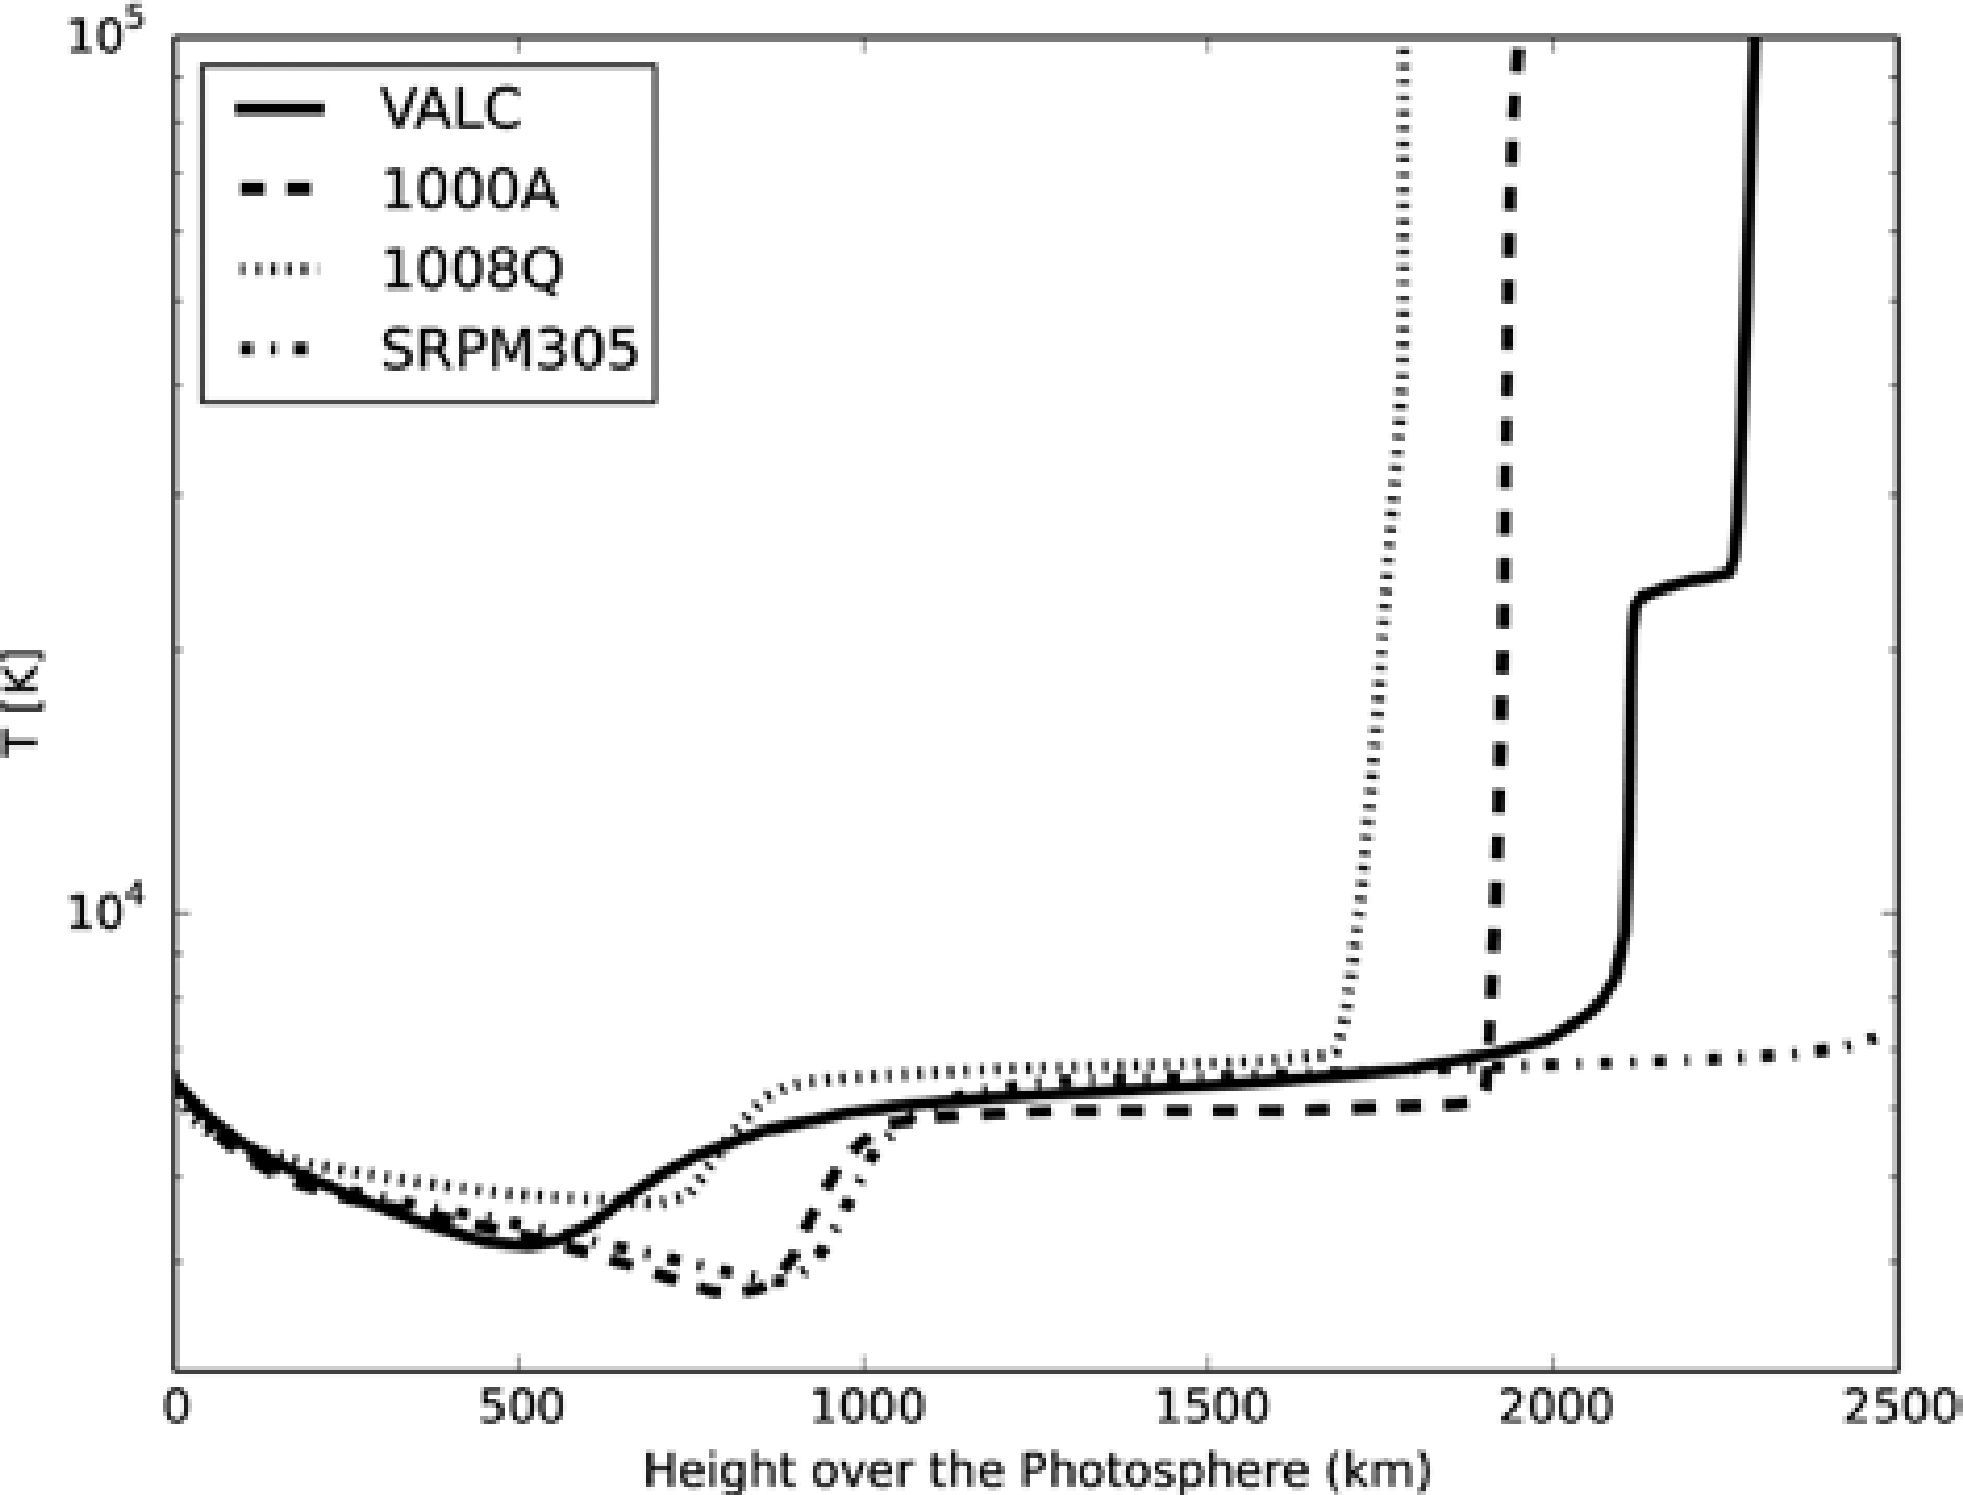
\includegraphics[width=\linewidth]{temperature_profile}
    \caption{Perfil de temperatura}
  \end{subfigure}
  \begin{subfigure}[b]{0.4\linewidth}
    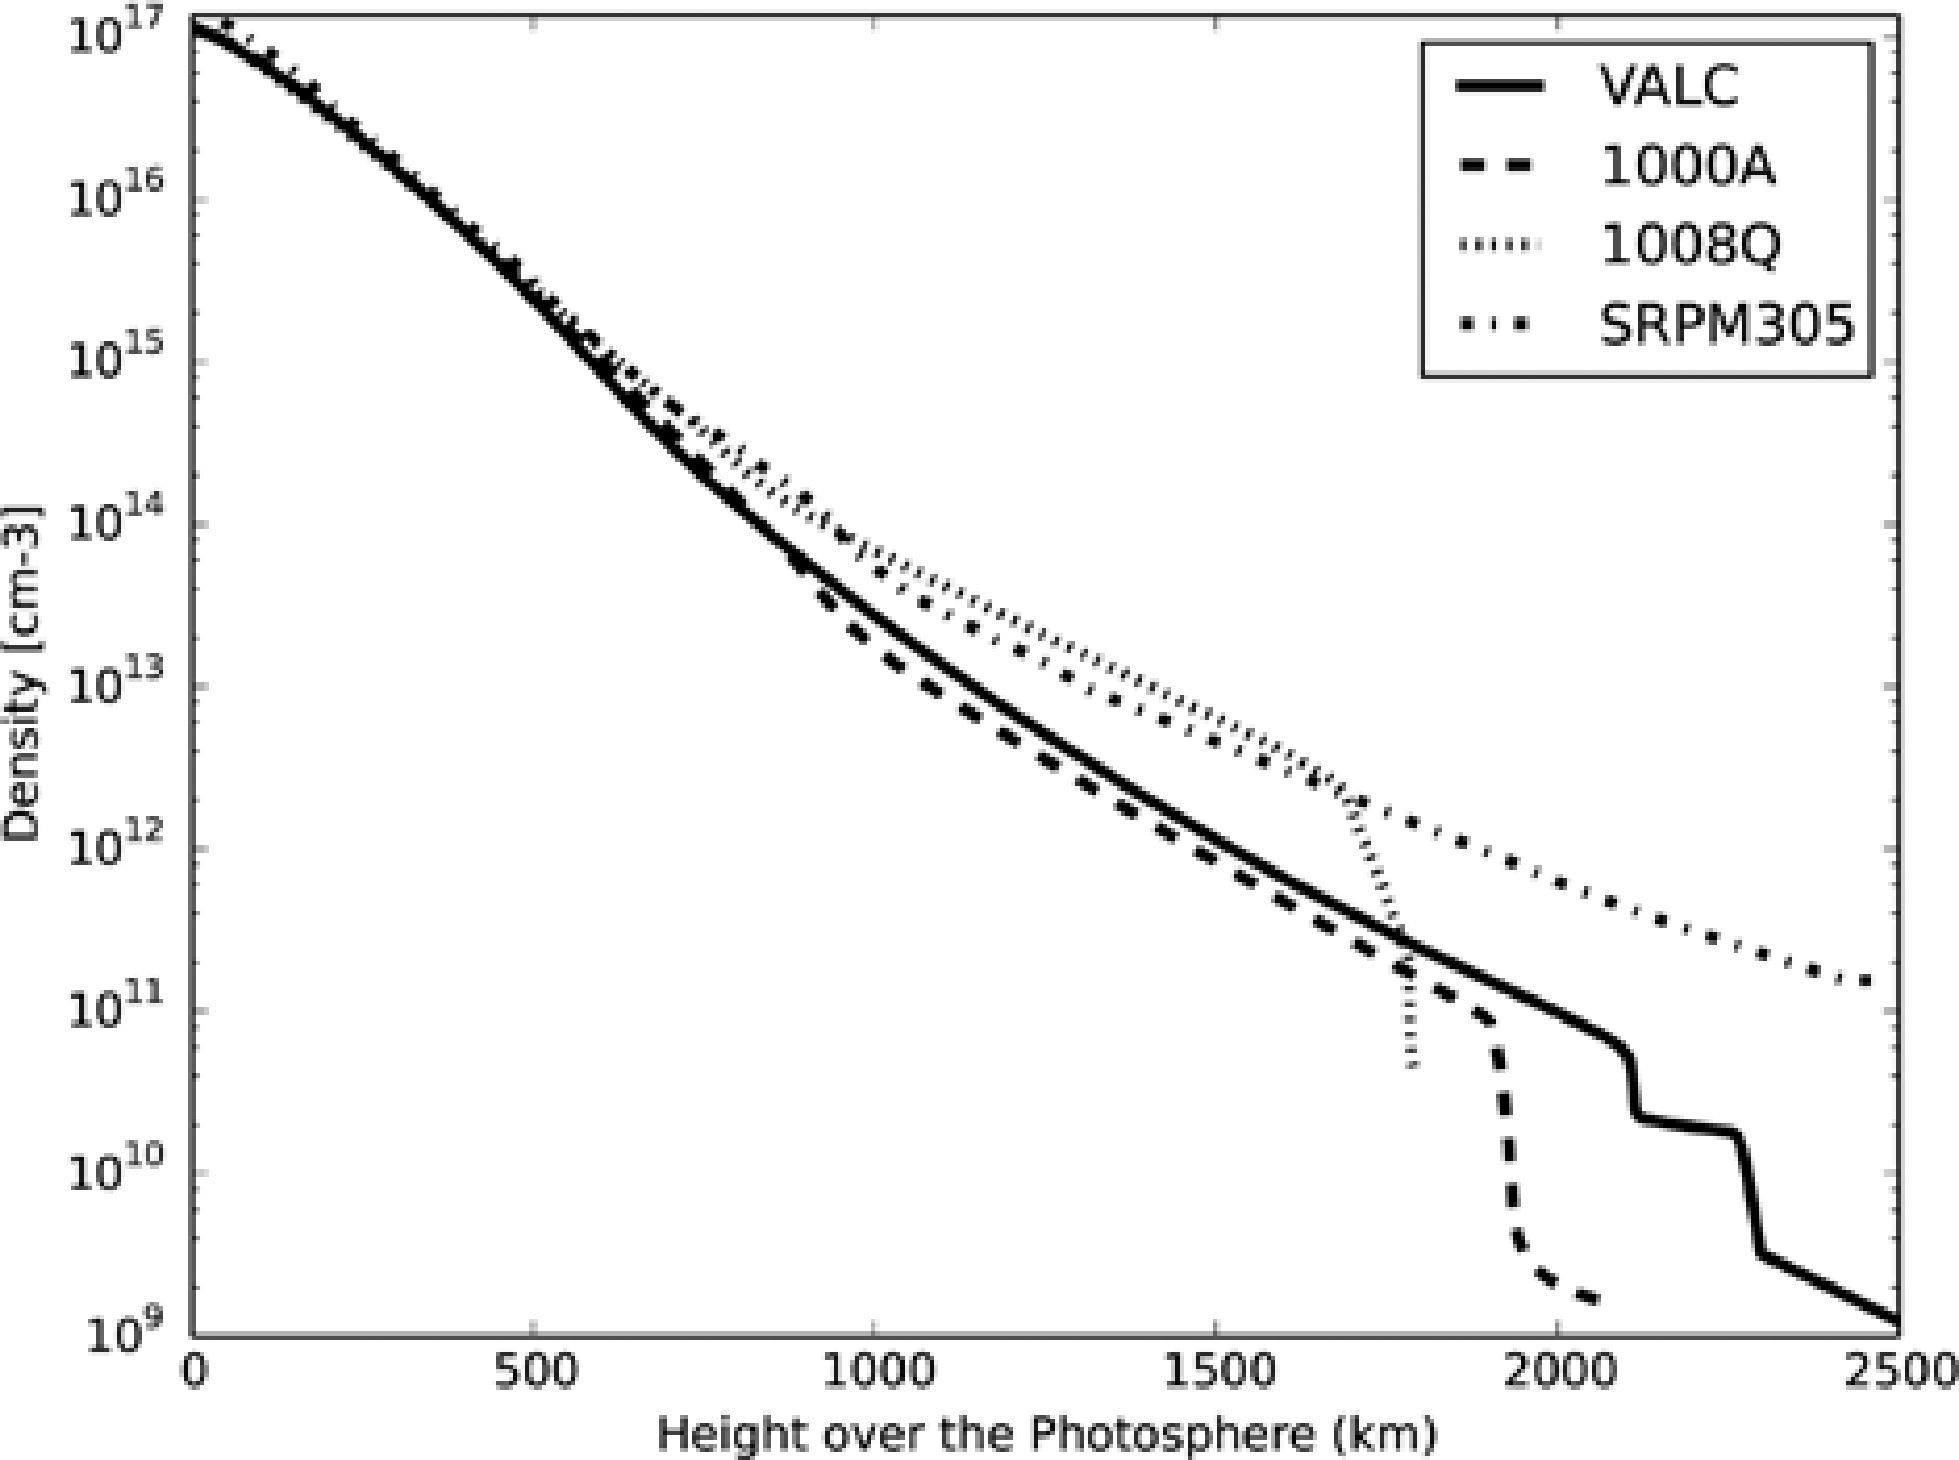
\includegraphics[width=\linewidth]{density_profile}
    \caption{Perfil de densidades}
  \end{subfigure}
  \caption{ (a) Perfiles de temperatura para los modelos VALC, SRPM305, 1000A y 1008Q los cuales muestran un m\'inimo de temperatura entre los 100 y 1000~km de altitud sobre la fot\'osfera. (b) Perfiles exponenciales de densidad que parte desde niveles fotosf\'ericos hasta altitudes alrededor del valot m\'inimo de la temperatura.}
  \label{semi_emp}
\end{figure}




Esta tesis extiende el estado del arte de la f\'isica solar mediante dos principales contribuciones. La primera contribuci\'on reside en proveer evidencia parcial y exploratoria, a trav\'es de una simulaci\'on computacional,  que las variaciones repentinas y radicales de la crom\'osfera se deben al efecto de los campos magn\'eticos de los niveles cromosf\'ericos y coronales. La segunda contribuci\'on consiste en complementar un modelo de simulaci\'on computacional existente para que considere el efecto de los campos magn\'eticos mismos. Con relaci\'on a esta segunda contribuci\'on, se refiere al modelo de simulaci\'on computacional llamado \emph{Pakal}, empleado para diagnosticar la emisi\'on milim\'etrica y submilim\'etrica proveniente de niveles coronales~\citep{2010ApJS..188..437D} con una resoluci\'on espacial comparable con la alcanzada con el instrumental actual.

Este c\'odigo est\'a escrito en C/MPI con licencia GNU/GPL. \emph{Pakal}MPI toma como dato de entrada, el perfil de densidad del Hidr\'ogeno, temperatura y metalicidad; calcula las abundancia en Equilibrio Termodin\'amico  Local (ETL) para 18 \'atomos y las abundancias de H, H$^{-}$ y electrones para fuera de ETL (NETL). Luego, calcula la trayectoria del haz y resuelve las ecuaciones de transferencia radiativa usando integraciones a lo largo de dicha trayectoria en segmentos cuya longitud es controlada por un algoritmo inteligente. La soluci\'on de la ecuaci\'on de transferencia depende de la profundidad \'optica a trav\'es de tres funciones distintas: Bemsstrahlung, H$^{-}$ y Bremsstrahlung inverso. Finalmente la temperatura de brillo la profundiad \'optica y las opacidades se registran en la proyecci\'on radial de cada paso.

Actualmente, el c\'odigo de Pakal realiza sus modelos de simulaci\'on sin considerar el efecto de los campos magn\'eticos en el c\'alculo de la densidad del plasma emisor de la crom\'osfera. Esto ocasiona que sus resultados sobre la densidad no sean del todo precisos en comparaci\'on con las observaciones reales. Mediante la extensi\'on del c\'odigo propuesta en esta tesis, se le posibilita a Pakal la capacidad de considerar el efecto de los campos magn\'eticos. Como resultado, sus aproximaciones a la densidad observada son m\'as precisos. Lo anterior permite robustecer el conocimiento de las variaciones repentinas y radicales observables en la temperatura de la crom\'osfera a partir de par\'ametros de la estructura magn\'etica tridimensional.


\mainmatter
\chapter{Estructuras de micro-escala en la crom\'osfera solar}

La atm\'osfera solar se divide en las siguientes capas: la fot\'osfera, crom\'osfera, regi\'on de transici\'on y la corona solar. Cada una de estas regiones poseen distintos reg\'imenes de densidad y temperatura ilustr\'andose en la Figura \ref{atmosfera_solar}.

\begin{figure}[ht]
\centering
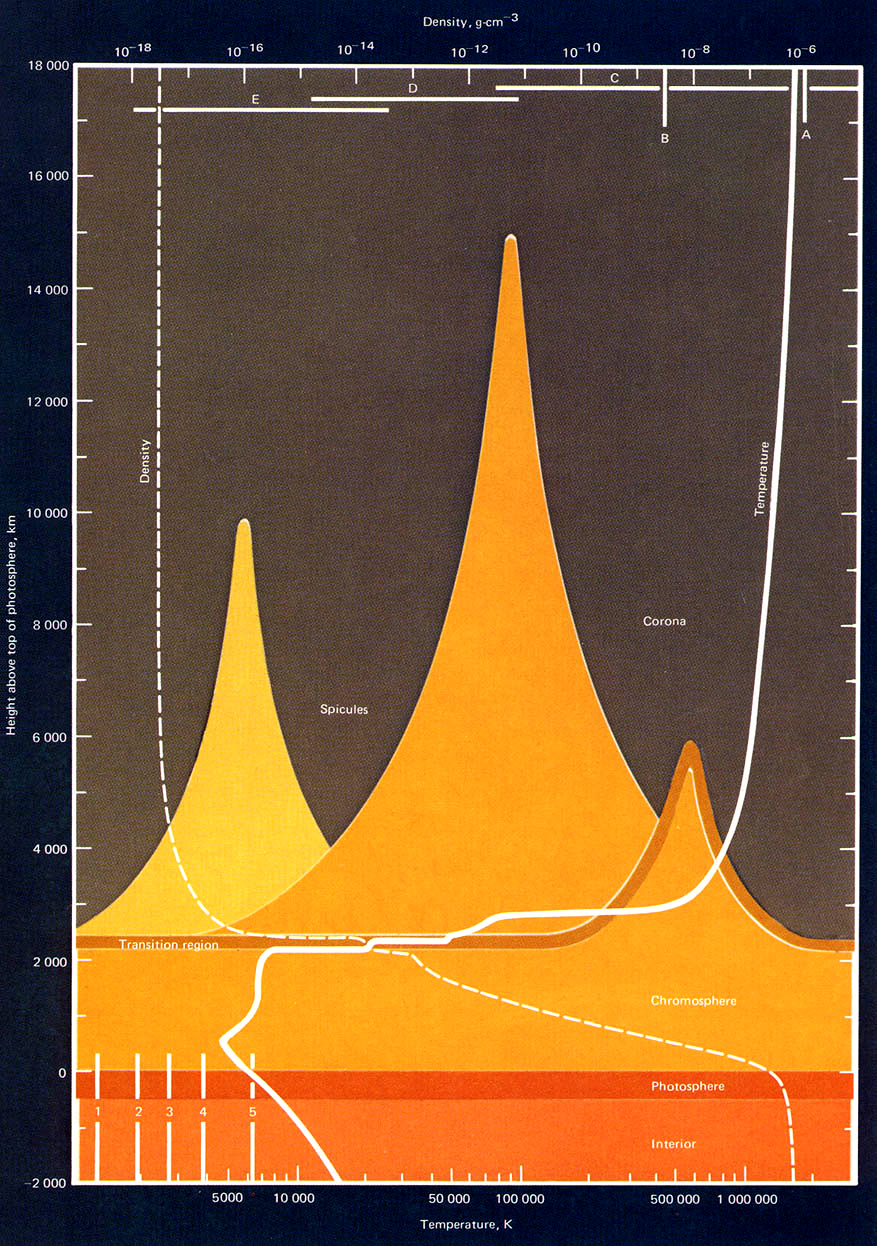
\includegraphics[scale=.65]{atmosfera_1}
\caption{Ilustraci\'on de la estructura de la atm\'osfera del Sol (tomada de https://history.nasa.gov/SP-402/p2.htm). \newline
*Existe debate sobre si la regi\'on de transici\'on es una regi\'on por s\'i misma o forma parte de la Crom\'osfera. Independientemente de esto, se localizar\'ia entre la Crom\'osfera y la Corona Solar.} \label{atmosfera_solar}
\end{figure}

Esta atm\'osfera solar est\'a descrita por la f\'isica de un plasma magnetizado. El estado del plasma y/o su interacci\'on con el campo magn\'etico establecen mecanismos de emisi\'on en pr\'acticamente todo el espectro electromagn\'etico. Estos mecanismos consisten en transiciones at\'omicas (que pueden ser ionizantes, de recombinaci\'on y tipo ligado-ligado) y mecanismos de emisi\'on libre-libre como radiaci\'on \emph{bremsstrahlung}, radiaci\'on sincrotr\'onica y radiaci\'on plasma.  ~\citep{ashwanden}

La atm\'osfera solar se extiende desde los niveles fotos\'ericos hasta el medio coronal pasando por el medio cromosf\'erico, involucrando una escala de longitud de $1R_{\odot}$--$3R_{\odot}$ ~\citep{NASAsun}. La \emph{fot\'osfera} se constituye de gr\'anulos convectivos de peque\~na escala ($10^3$~km), separados de entre s\'i por capas intergranulares, las cuales concentran elementos de alto flujo magn\'etico ($|B| \le 1\mbox{kG}$). La escala temporal de la ocurrencia de un gr\'anulo es de unos minutos aproximadamente. La \emph{crom\'osfera} (ver Figura \ref{atmosfera_solar}) es una capa que se extiende por alrededor de $2\times 10^3$~km. Emite intensamente en la l\'inea H$\alpha$ ($\lambda=6563~\mbox{\AA}$) y ultravioleta. Similarmente a la fot\'osfera, la base de la crom\'osfera presenta gr\'anulos con una escala de tama\~no relativamente mayor concentrando flujo magn\'etico, el cual est\'a asociado en unos casos con flujos verticales de plasma llamados \emph{esp\'iculas} o a microarcos magn\'eticos en otros casos ~\citep{NASAweb}. M\'as all\'a de la base de la crom\'osfera cambia la condici\'on en la presi\'on dominante, ya que mientras la presi\'on del gas domina a niveles fotosf\'ericos, a estos niveles esta condici\'on se invierte y las distribuciones de brillo observadas est\'an dominadas por la geometr\'ia del campo magn\'etico ~\citep{priest}.

%Por su parte, la \emph{corona} es una de las partes de la atm\'osfera m\'as desconocidas para la ciencia hasta el momento. Su mayor misterio es que conforme la densidad decrementa, la temperatura en lugar de decrementar tambi\'en se incrementa. Este fen\'omeno se presenta a\'un m\'as radicalmente en una capa que antecede a la Corona conocida como la regi\'on de transici\'on (TR por su nombre en ingl\'es "Transition Region"). Particularmente, en dicha regi\'on a\'un no est\'a claramente explicado el cambio radical que pasa de $10^4$K a $10^5$ K en una distancia de $1000$~km (v\'ease fig.~\ref{atmosfera_solar}).

El rango de temperaturas implicado en este cambio de morfolog\'ia, de gr\'anulos a estructuras filamentarias magn\'eticas (\emph{en ingl\'es loops}) es de $2\times 10^5~\mbox{K} < T < 10^6~\mbox{K}$. Este escenario anterior propone que, a trav\'es de las ep\'iculas se establece un mecanismo continuo de transferencia de material y energ\'ia hacia la corona solar, por lo que se han propuesto modelos que expliquen tanto la din\'amica y estructura t\'ermica de una condici\'on conocida como \emph{Sol Quieto}, en referencia a regiones del Sol que excentas de cualquier manifestaci\'on de actividad observable \citep{ashwanden}. Modelos est\'aticos de atm\'osferas referentes, son los desarrollados por Vernazza et al. 1991 (VAL), Fontenla et al. 1993 y Avrett y Loeser 2008 (C7). En ellos, se ajusta una atm\'osfera hidrost\'atica, promediando propiedades estratificadas en una aproximaci\'on plano-paralela hasta reproducir el correspondiente espectro emergente para un conjunto de observaciones seleccionadas. A\'un cuando la f\'isica de aquellos modelos es bastante realista, no toma en cuenta la din\'amica a escala angular menor al poder de resoluci\'on angular de las observaciones actuales.

Con el advenimiento de instrumentos que observan en el rango UV, como el Interface Region Imaging Spectrograph (IRIS) y el Solar Dynamics Observatory (SDO), muestra que la estructura de la atm\'osfera (y muy particularmente, de la crom\'osfera) es tan complejamente distribuida, que un modelo que promedie propiedades como en el p\'arrafo anterior no puede capturar el escenario real ~\citep{VAULT1}. 

En a\~nadidura, las  observaciones del experimento VAULT (Very high Angular resolution ULtraviolet Telescope por sus siglas en ingl\'es) complementan la evidencia de una estructura cromosf\'erica y de la existencia de peque\~nos loops frios \citep{VAULT1}, los cu\'ales confirman la presencia de campos magn\'eticos.
VAULT es un proyecto de exploraci\'on espacial que data de 1999 y que busca estudiar la conexi\'on entre la corona y la crom\'osfera solar al observar la l\'inea espectral m\'as fuerte del sol, la Ly$\alpha$ a 1216~$\mbox{\AA}$.
La resoluci\'on angular de sub-arcosegundos ($\approx$.3") permite ver directamente los peque\~nos loops f\'ios en la estructura de Sol Quieto. El parecido de los resultados entre los modelos y las observaciones indican que la explicaci\'on de las estructuras finas observadas en t\'erminos de loops frios es plausible.

Como se muestra en la Figura \ref{fig:vault_compare} las im\'agenes de VAULT nos permiten mejorar la calidad de nuestras observaciones, permiti\'endonos tener un mejor entendimiento de la composici\'on de la atm\'osfera solar (n\'otese tambi\'en la calidad de la Figura \ref{fig:vault_complete}) ~\citep{VAULT1}.

\begin{figure}[ht]
\centering
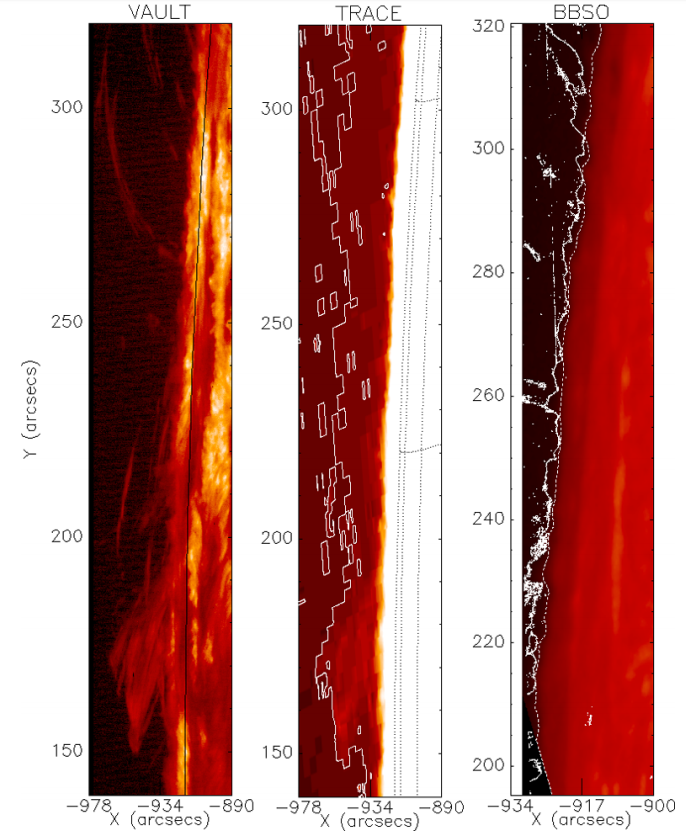
\includegraphics[scale=0.6]{vault_comparison}
\caption{Comparaci\'on realizada entre distintas observaciones, mostrando la resoluci\'on de las im\'agenes tomadas por el proyecto VAULT}
\label{fig:vault_compare}
\end{figure}

\begin{figure}[ht]
\centering
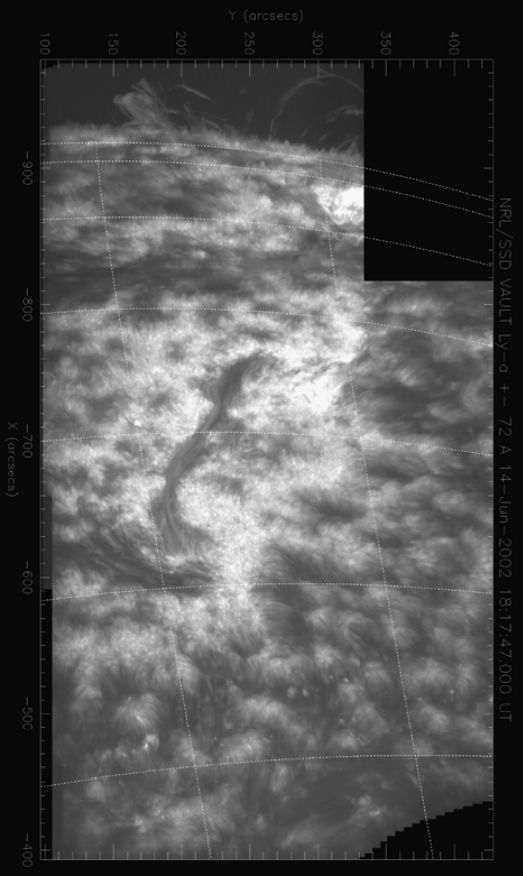
\includegraphics[scale=0.6]{vault_complete}
\caption{Imagen construida a partir de observaciones realizadas por el proyecto VAULT}
\label{fig:vault_complete}
\end{figure}

Actualmente se esta develando la estructura en el disco solar en ondas mm ($\lambda=3$~mm) con una resoluci\'on 3.7'' $\times$ 2.5''\citep{2018A&A...619L...6N}. La distribuci\'on de brillo es muy similar a la observada en su contraparte ultravioleta por el sat\'elite IRIS (ver Figura ~\ref{fig:chromosphericnet1}): una red cromosf\'erica constitu\'ida de gr\'anulos con temperatura de brillo $T_{b}=6500$~K en promedio (\citep{2018A&A...619L...6N}). Lo anterior sugiere que la radioemisi\'on en ondas mm esta  ubicada en la regi\'on cromosf\'erica dispuesta en flujos emergentes o estructuras filamentarias observadas al limbo (loops) (ver Figura ~\ref{fig:chromosphericnet2})

Se puede decir entonces que el conocimiento con respecto al impacto de las micro estructuras magn\'eticas en la emisi\'on milim\'etrica y submilim\'etrica es escaso. Sin embargo existen esfuerzos recientes por comprender este impacto. Por ejemplo, \emph{Pakal} (De la Luz 2010) es un c\'odigo que resuelve la ecuaci\'on de transferencia radiativa en tres dimensiones en una aproximaci\'on plano-paralela, cuya estratificaci\'on sigue perfiles conocidos de densidad y temperatura y bas\'andose de los modelos semi-emp\'iricos VAL y C7, lo cuales, bajo determinadas modificaciones se introducen en c\'odigo \emph{Pakal}.

\begin{figure}[ht]
\centering
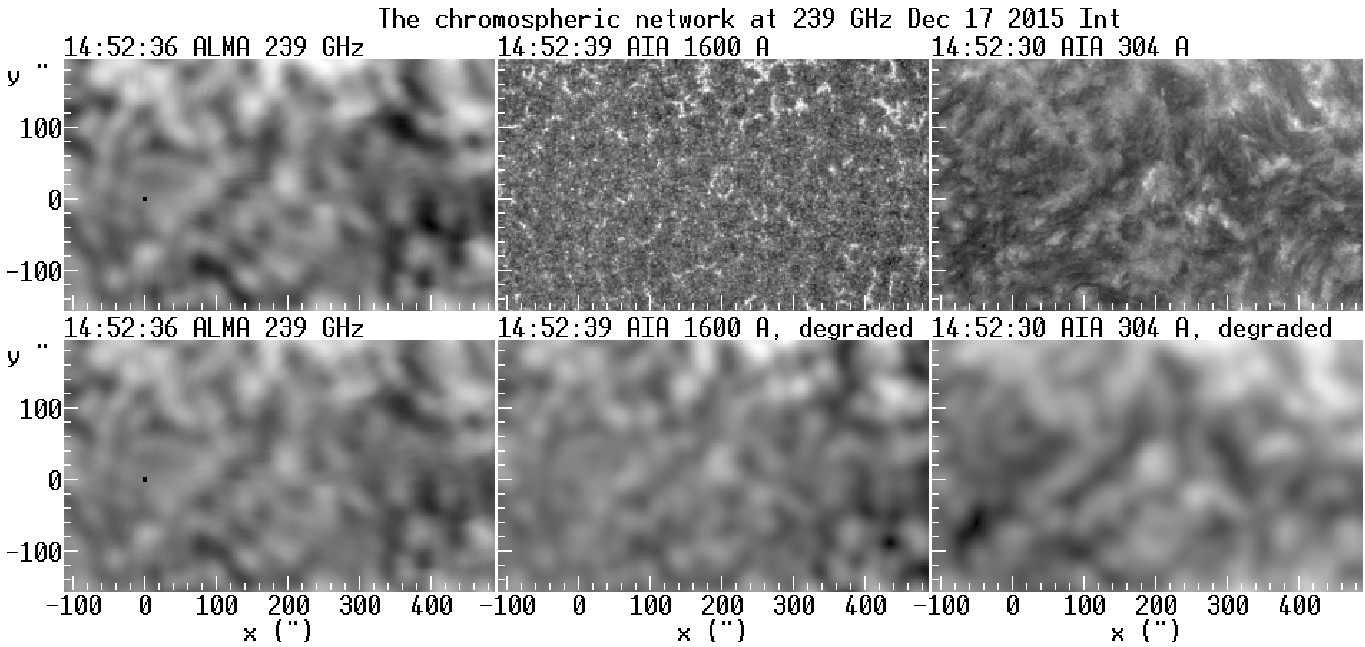
\includegraphics[scale=0.4]{ALMA}
\caption{Im\'agenes de la red cromosf\'erica en las cercan\'ias del centro del disco solar durante el 17 de Diciembre de 2015 a 239~GHz (1.2~mm) junto con im\'agenes de AIA-SDO a 1400~$\mbox{\AA}$ (continuo) y 304~$\mbox{\AA}$ (emisi\'on de HeII). En el rengl\'on de abajo se muestran las im\'genes de AIA-SDO degradadas a las resoluci\'on de ALMA~\citep{2017A&A...605A..78A}.}
\label{fig:chromosphericnet1}
\end{figure}

\begin{figure}[ht]
\centering
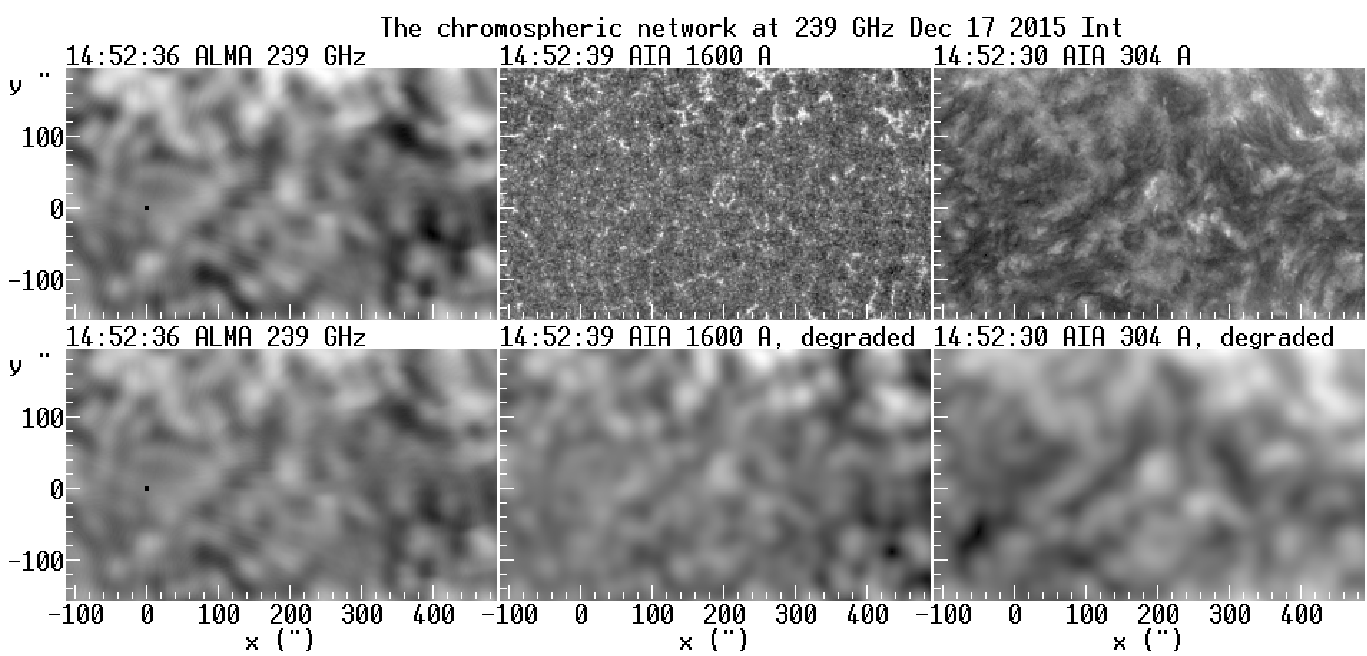
\includegraphics[scale=0.4]{ALMA_I}
\caption{Im\'agenes de ALMA mostrando el disco completo durante el 17 de Diciembre de 2015 comparadas con im\'agenes en otras longitudes de onda. \emph{Arriba de izquierda a derecha: }im\'agen de ALMA a 239~GHz; la misma pero degradada a la resoluci\'on de la im\'agen de 100~GHz; e ima\'agen de ALMA a 100~GHz sin degradar. \emph{Rengl\'on inferior: } H$\alpha$ de la red GONG; im\'agen a 1600~$\mbox{\AA}$ de AIA-SDO; y magnetograma de HMI-SDO~\citep{2017A&A...605A..78A}.}
\label{fig:chromosphericnet2}
\end{figure}

%\begin{figure}[ht]
%\centering
%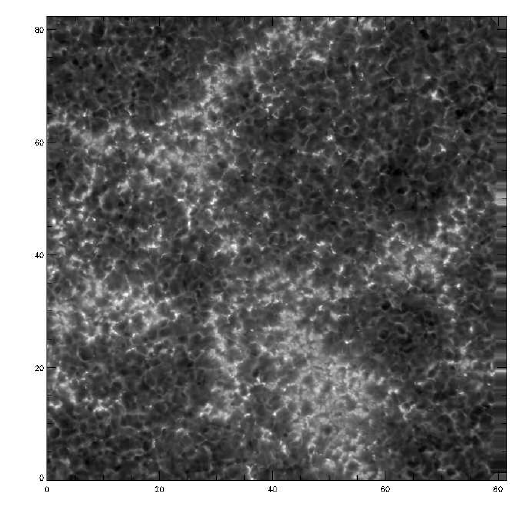
\includegraphics[scale=0.5]{chromospheric_network2}
%\caption{ Red cromosf\'erica solar observada desde el Telescopio Solar Sueco (Swedish Solar Telescope) en la l\'inea H Ca II.
%\newline Fuente: https://www.researchgate.net/figure/The-chromospheric-network-as-observed-with-the-Swedish-Solar-Telescope-in-the-Ca-II\_fig8\_259104617}
%\label{chromospheric_network2}
%\end{figure}



%En la figura \ref{fig:chromosphericnet} se observa una imagen tomada en la l\'inea de c\'alcio de la red cromosf\'erica, mientras que en la figura 

\section{El c\'odigo \emph{Pakal}}
%Descripci\'on del c\'odigo, puntualmente hay qu\'e explicar primero para qu\'e sirve actualmente y a partir de ello, plantear las modificaciones.
Como se mencion\'o anteriormente, esta tesis busca extender el c\'odigo Pakal 2011\citep{Pakal}. Dicho programa es un modelo num\'erico inovador que pretende resolver la ecuaci\'on de transferencia radiativa en una geometr\'ia tridimensional (3D), usando una aproximaci\'on para una atm\'osfera localmente plano paralelo; lo anterior utilizando un sistema inteligente. Con este programa se generan las capas estratificadas de la atm\'osfera en una estructura l\'ogica. La salida del c\'odigo puede ser en forma de mapas bi-dimensionales o un perfil de una dimensi\'on, que reproduce las observaciones con alta presici\'on, dando informaci\'on f\'isica detallada acerca del entorno donde la radiaci\'on fue generada y/o transmitida.

Pakal se encuentra dividido en cuatro distintos m\'odulos: El modelo num\'erico, la geometr\'ia, los m\'etodos num\'ericos y las funciones f\'isicas. Estos cuatro m\'odulos pueden ser modificados independientemente sin afectar el funcionamiento de los otros. En esta tesis se modifica el m\'odulo de las funciones f\'isicas donde se resuelve la ecuaci\'on de transferencia.

Como todo modelo, Pakal est\'a basado en una serie de supuestos que le brindan una serie de fortalezas, pero tambi\'en una serie de limitantes; las cuales se presentar\'an a continuaci\'on. Con relaci\'on a sus supuestos, Pakal presenta un modelo aplicado a una geometr\'ia solar radial 3D, asumiendo una atm\'osfera local plano-paralela, y una emisi\'on t\'ermica de radio libre-libre de gas hidr\'ogeno-helio en equilibrio termodin\'amico. Para sus c\'alculos Pakal asume un grosor de la Crom\'osfera de 2200km. Adem\'as tambi\'en utiliza perfiles radiativos precalculados de densidad y temperatura (basado en modelos hidrost\'aticos, hidrodin\'amicos o MHD) para calcular la emisi\'on de una fuente de estructuras 3D con alta resoluci\'on espacial. En todo momento Pakal asume un estado de Sol Quieto y la ausencia de campos magn\'eticos. El t\'ermino Sol Quieto hace referencia a regiones del Sol que se encuentran excentas de cualquier manifestaci\'on de actividad observable. Pakal resuelve la ecuaci\'on de transferencia radiativa en un conjunto de l\'ineas dirigidas de la fuente al observador.

En relaci\'on con las limitaciones de Pakal, si bien este permite la entrada de observaciones, no est\'a basado en ellas, y por lo tanto los resultados no representan por completo las caracter\'isticas f\'isicas existentes. De igual forma, Pakal se encuentra limitado a la crom\'osfera. Adem\'as Pakal omite la emisi\'on \emph{gyrosynchrotron} al despreciar los campos magn\'eticos. Finalmente, el c\'odigo de Pakal no logra reproducir en un 100\% las funci\'ones de densidad y temperatura del plasma solar.
 
Pakal ha demostrado poder mejorar el tiempo de integraci\'on hasta por un orden de magnitud comparado a c\'odigos de integraci\'on lineal. Por ejemplo, en una prueba que utilizaba 32 procesadores de una m\'aquina Cray del CNS en san Luis Potos\'i, se generaron espectros sint\'eticos de 32 frecuencias, con pasos de integraci\'on de 1km del centro del disco solar en aproximadamente 3 segundos. Adem\'as, Pakal puede correr en clusters, supercomputadoras y computadoras personales. Los resultados de Pakal han sido probados por su robustez. Particularmente, se realizaron satisfactoriamente pruebas de convergencia y estabilidad de la parte num\'erica y del sistema experto, las cu\'ales son presentadas en De la Luz et al. (2010). Por \'ultimo, Pakal permite modelar computacionalmente modelos semi emp\'iricos. 

En esta tesis se propone una extensi\'on en el m\'odulo de funciones f\'isicas (denominado Jaguar). Particularmente se agrega el efecto de los campos magn\'eticos a la ecuaci\'on de transferencia al agregar la componente de la presi\'on magn\'etica. Lo anterior convierte al modelo hidrodin\'amico que se usa actualmente en un modelo magnetohidrost\'atico. Con esta adici\'on (1) se puede generar un escenario m\'as apegado a las observaciones f\'isicas de la atm\'osfera solar, y (2) se facilita la adaptaci\'on del c\'odigo ante la adici\'on de cualquier modelo de campo magn\'etico.



\section{Sobre el Sol quieto y la emisi\'on submilim\'etrica solar}

El concepto de emisión de radio del sol quieto se refiere a una simplifiación teórica en la cantidad de emisión de radio del Sol. Sin embargo, el Sol nunca se encuentra por completo quieto; algunos procesos turbulentos en la atm\'osfera solar y la corona hacen aparentar que existen regiones cuya emisi\'on de radio, siendo naturalmente espor\'adica, incrementa el valor de su intensidad observada cuando es comparada con el nivel "quieto" del Sol ~\citep{sol_quieto}.

En este trabajo, se asume \'unicamente el estado de sol quieto debido a la complejidad del Sol activo. Sin embargo, el entendimiento del sol quieto tambi\'en nos ayudar\'ia a entender mejor el Sol Activo. Concretamente, la correcta caracterizaci\'on del Sol Quieto nos permitir\'ia entender el excedente de radiaci\'on que se le atribuye al Sol Activo.

Una caracter\'istica relevante del Sol quieto para esta tesis es la intensidad de sus campos magn\'eticos. Particularmente los campos magn\'eticos del sol quieto, medidos seg\'un las l\'ineas espectrales de Zeeman, contienen un campo de B= .1 - .5G, mientras que sus fuerzas absolutas de campo en elementos espacialmente resueltos var\'ian entre B = 10-50G \citep{1000G}. Estos valores se utilizan en el modelo computacional propuesto en este texto.

Si bien se conocen los rangos de la magnitudes de los campos magn\'eticos del sol quieto ~\citep{VAULT2}, existe una dificultad en medir las magnitudes concretas de estos debido a corrientes desconocidas y condiciones de fuerza no libre. Lo anterior ocasiona que se tengan que calcular extrapolaciones a lo largo de la crom\'osfera y la regi\'on de transici\'on para obtener valores aproximados. 

La región de transición es una capa muy delgada e irregular de la atmósfera solar que separa la corona caliente de una cromósfera mucho más fría. El calor fluye de la corona a la cromósfera en un proceso que produce esta pequeña regi\'on donde la temperatura cambia rápidamente de $10^6$~K hasta $2\times 10^5$~K. A esas temperaturas, el hidrógeno es ionizado, provocando que la luz emitida en esta región sea dominada por iones como C IV, O IV y Si IV (Carbono, Oxígeno y Silicio); emitiendo luz en la región ultravioleta del espectro solar ~\citep{NASAtr}%, es la de la nasa NASA 2014.
%(solarscience.msfc.nasa.gov/t_region.shtml)

Otra caracter\'istica importante del sol quieto para esta tesis es la emisi\'on milim\'etrica del plasma. Con la emisi\'on milim\'etrica se puede aproximar el grado de ionizaci\'on de la atm\'osfera solar; y se pueden inferir aproximaciones de la temperatura, la densidad y la presi\'on que hay en ella ~\citep{millimeter}. Estas \'ultimas aproximaciones se realizan seg\'un diferentes modelos; los cuales se pueden conceptualizar como emp\'iricos, semi-emp\'iricos y observacionales ~\citep{2010ApJS..188..437D}.

Independientemente del tipo de modelo, por definici\'on, todos tienen limitaciones en sus c\'alculos de temperatura, densidad y presi\'on. En el modelo propuesto, se busca robustecer el modelo Pakal mediante la anexi\'on de el efecto te\'orico de los campos magn\'eticos. Esta anexi\'on se puede justificar, por diferentes teor\'ias y observaciones. Por ejemplo, un estudio reciente por Meunier (2018) propone que las peque\~nas regiones de campo magn\'etico contribuyen a la emisi\'on cromosf\'erica y por consiguiente a la emisi\'on milim\'etrica. Lo anterior, como se explic\'o previamente, afectar\'ia a los c\'alculos de la temperatura, la densidad y la presi\'on de la crom\'osfera; haci\'endolos te\'oricamente m\'as precisos.

A continuaci\'on se define la temperatura de brillo $T_{b}$, temperatura efectiva $T_{\mbox{\tiny eff}}$ y las relaciones de la transferencia radiativa en una forma que \'util para la interpretaci\'on de las observaciones de radio de acuerdo a~\citep{dulk_stars}.

Para un material que est\'a en \emph{equilibrio termodin\'amico}, la intensidad $I_{\nu}$ de su campo de radiaci\'on, equivale a la distribuci\'on de energ\'ia
$B_{\nu}(T)$que caracteriza al mismo. En particular, para el r\'egimen de Rayleigh-Jeans donde $h\nu \ll k_{B}T$, La intensidad $I_\nu$ se relaciona con $T_{b}$, para un medio \'opticamente grueso, mediante:

\begin{equation} \label{temperatura_brillo}
I_\nu = kT_bv^2/c^2\, erg \, cm^{-2} \,s^{-1} \,Hz^{-1} \,sr^{-1}
\end{equation}


Y la ecuaci\'on de transporte radiativo

\begin{equation}
\frac{dI_{\nu}}{d\tau_{\nu}}=-I_{\nu}+S_{\nu}
\end{equation}  

Se expresa como:
\begin{equation} \label{diferencial_temperatura}
dT_b/d\tau_\nu = -T_b + T_{eff}
\end{equation}

Donde la \emph{funci\'on fuente} $S_{\nu}$ satisface:

\begin{equation} \label{fuente}
S_\nu = B_{\nu}(T_{\mbox{\tiny eff}})=kT_{\mbox{\tiny eff}}\nu^2/c^2
\end{equation}

En contraste, para una distribuci\'on no t\'ermica, $T_{\mbox{\tiny eff}}$ generalmente es una funci\'on tanto de frecuencia como de modo de polarizaci\'on (Wild et al. 1963). Entonces, la soluci\'on para la temperatura de brillo es:

\begin{equation} \label{temperatura_integral}
T_{b} = \int_{0}^{\tau_\nu} T_{\mbox{\tiny eff}} e^{-t_\nu} dt_\nu + T_{b0} e^{-\tau_\nu}
\end{equation}

Para el caso especial de una fuente aislada con $T_{eff}$ constante, la ecuaci\'on \ref{temperatura_integral} se reduce a

\begin{equation} \label{t_brillo1}
T_{b} = T_{\mbox{\tiny eff}}[1-e^{-\tau_\nu}]
\end{equation}

\begin{equation} \label{t_brillo2}
T_{b} = T_{\mbox{\tiny eff}} \qquad (\mbox{si} \, \tau_\nu \gg 1)
\end{equation}

\begin{equation} \label{t_brillo3}
T_{b} = T_{\mbox{\tiny eff}} \tau_\nu (c^2/k\nu^2)\eta_ \nu L \qquad (\mbox{si} \, \tau_\nu \ll 1)
\end{equation}


Para radiaciones incoherentes, las ecuaciones \ref{t_brillo1} y \ref{t_brillo2} son de considerable importancia y utilidad. Ah\'i se muestra que tal radiaci\'on no puede alcanzar un valor de $T_{\mbox{\tiny b}}$ m\'as alto que $T_{\mbox{\tiny eff}}$. Adem\'as, la funci\'on fuente $T_{\mbox{\tiny eff}}$ se relaciona con la energ\'ia media de las part\'iculas que emitidas por $\langle E \rangle$ = $k_{\mbox{\tiny B}}T_{\mbox{\tiny eff}}$. Por ejemplo, para electrones monoel\'ectricos de $T_{\mbox{\tiny eff}}$ = $E_0/k$ o una distribuci\'on Maxweliana de $T_{eff}$ = $T$ = $E_0/k$, tenemos que $T_{\mbox{\tiny b,max}} = T_{\mbox{\tiny eff}}$, por ejemplo $T_{\mbox{\tiny b,max}} = 1.16 \times 10^7$ K si $E_0 = 1$~keV \'o $1.16 \times 10 ^{10}$~K si $E_0 = 1$MeV. En el caso de una distribuci\'on elect\'onica en ley de potencias, $T_{eff}$ se determina por la energ\'ia media de los electrones que contribuyen principalmente a la intensidad a una frecuencia en particular (y un modo de polarizaci\'on). Si esa energ\'ia media y por lo tanto la temperatura de brillo son muy altas, las circunstancias  deben ser que la mayor cantidad de electrones de baja energ\'ia no emitan y absorban eficientemente; en general, esto requiere un campo magn\'etico d\'ebil. Bajo condiciones estelares y solares, la fuerza de los campos tiende a ser grande y las energ\'ias electr\'onicas bajas (comparado por ejemplo, con fuentes extragal\'acticas), tal que $T_{\mbox{\tiny eff}}$ y $T_{\mbox{\tiny b}}$ de emisi\'on incoherente poseen valores limitados entre $10^9$ y $10^{10}$~K. Valores superiores observados, implican un mecanismo coherente, tal como un maser o radiaci\'on plasma.
La densidad de flujo S (para una polarizaci\'on) de una fuente de radio se relaciona con la temperatura de brillo mediante:

\begin{equation} \label{densidad_flujo}
S = k_{\mbox{\tiny B}}\nu^2/c^2 \int T_{\mbox{\tiny b}} d\Omega
\end{equation}

donde $d\Omega$ es un elemento diferencia de \'angulo s\'olido y la integral es sobre el \'area proyectada de la fuente.

Cuando los electrones son desviados individualmente en los campos coulombianos de iones debido a su movimiento acelerado, se produce bremsstrahlung, o emisi\'on libre-libre. El proceso inverso, absorci\'on libre-libre, ocurre cuanddo los electrones comienzan a oscilar en resonancia con el campo el\'ectrico de una onda. Eventualmente las colisiones electr\'on-i\'on destruyen esta oscilaci\'on diezmando la energ\'ia de la onda y calentando por consecuencia el plasma.

El coeficiente de absorci\'on para electrones t\'ermicos es

\begin{equation*} \label{coeficiente1}
\kappa \approx \sum_{i} \frac{1}{3c} \left(\frac{2}{\pi}\right)^{1/2} \frac{\nu_p^2}{\nu^2} \frac{4\pi Z_i^2 n_i e^4}{m^{1/2}(kT)^{3/2}} \frac{\pi}{\sqrt{3}}G(T,\nu)
\end{equation*}
\begin{equation*} \label{coeficiente2}
\approx 9.78 \times 10^{-3} \frac{n_e}{\nu^2T^{3/2}} \sum_i Z_i^2 n_i
\end{equation*}
\begin{equation} \label{coeficiente_absorcion}
\times =
    \begin{cases}
    18.2+\mbox{ln} T^{3/2}-\mbox{ln}\nu    & (T < 2 x 10^5 \mbox{K})\\
    24.5+\mbox{ln}T-\mbox{ln}\nu           & (T < 2 x 10^5 \mbox{K}).
    \end{cases}
\end{equation}


La emissividad $\eta_\nu$ se encuentra relacionada a $\kappa_\nu$ por la ley de Kirchhoff:

\begin{equation}
\eta_{\nu}=B_{\nu}(T)\kappa_{\nu}
\end{equation}
 
Para varios casos una forma simplificada de la Ecuaci\'on \ref{coeficiente_absorcion} puede ser usada. Asumiendo un plasma hidr\'ogeno-helio completamente ionizado y tomando valores t\'ipicos de $\nu \sim 10^8$~Hz y $T \sim 10^6$~K para el t\'ermino logar\'itmico, tenemos

\begin{equation} \label{coeficiente_absorcion_simple}
\kappa \approx 0.2 n_e^2T^{-3/2} \nu^{-2}~\mbox{cm}^{-1}
\end{equation}

\chapter{Extensi\'on al modelo Pakal \-- A\~nadiendo presi\'on magn\'etica}

La extensi\'on propuesta en esta tesis al modelo computacional Pakal le a\~nade a este \'ultimo el efecto de la presi\'on magn\'etica a la ecuaci\'on de estado. Con lo anterior, el modelo de Pakal, que en principio era un modelo computacional que simulaba un modelo hidrost\'atico para el comportamiento del plasma, se robustece al convertirse en un modelo Magnetohidrost\'atico. El modelo original resuelve la siguiente ecuaci\'on de estado:

\begin{equation*} \label{ecuacion_hidrostatica}
\frac{dp}{dz} = g\rho
\end{equation*}
donde

\begin{equation*} \label{ecuacion_presion}
p = p_g + \frac{1}{2}\rho v_t^2
\end{equation*}
*agregar referencia y explicar que pedo*

A esta f\'ormula, se le a\~nade el efecto de la presi\'on magn\'etica, resultando en la siguiente ecuaci\'on\citep{priest}.

\begin{equation*} \label{mhs}
p = p_g + \frac{1}{2}\rho v_t^2 + p_B
\end{equation*}
*agregar referencia y explicar que pedo*

Cabe aclarar que la f\'ormula que utiliza el c\'odigo de la extensi\'on a Pakal considera la siguiente ecuaci\'on de presi\'on magn\'etica para realizar los c\'alculos:

$P_B = \frac{B^2}{8\Pi}$
*agregar referencia y explicar que pedo*

A continuaci\'on se precisar\'a el c\'odigo de la extensi\'on computacional al programa Pakal realizado en esta tesis. Se contextualizar\'a dicho c\'odigo con secciones del c\'odigo original. Las extensiones al c\'odigo se diferenciar\'an al c\'odigo original al estar con un estilo de letra en \textbf{negrita}, mientras que los nombres de los archivos se encuentran \underline{subrayados}. Adem\'as, se comentar\'a la funci\'on realizada por el c\'odigo agregado. 

Para hacer posible la adici\'on del efecto de la presi\'on magn\'etica sobre la ecuaci\'on de estado dentro del c\'odigo Pakal, se modificaron los siguientes archivos:\newline

\underline{hmodel.h}
En esta libreria se definen la estructura de la atmosfera, a la cual se le agregaron las componentes x, y, z del campo magnetico, asi como la variable $\xi$ para la modulacion del mismo
\begin{lstlisting}[style=CStyle]
typedef struct{
	int id;
	double z;
	double T;
	double P;
	double H;
	double V;
	double vt;
	double ne;
	double ne_lte;
	double bhm;
	double fz;
	/*-------------------------------------------------------------*/
	//Se agregan las componentes del campo y xi
	double Bx;
	double By;
	double Bz;
	double xi;
	/*-------------------------------------------------------------*/	
}Atmosphere;

\end{lstlisting}

\underline{main.c}
Esta es la parte donde el m\'odulo Jaguar se encarga de llamar a las respectivas funciones que llevan a cabo los c\'alculos de cada uno de los pasos de integraci\'on. En este c\'odigo se agreg\'o la lectura de los valores de campo.\newline
Los parametros amplitud e intensidad son los respectivos valores del campo magnetico.\newline
El par\'ameto alpha se define en el capitulo 4.\newline
El par\'ametro B\_x0 representa la altura a la que nace el campo magn\'etico, tomando como referencia la base de la fot\'osfera.
\begin{lstlisting}[style=CStyle]

int main(int argc, char **argv){
	int i,j;
	Model model;
	char env[500];
	char comando[500];
	double hydro_step;
	double pz1;
	double Y;
	double fz1;
	double dx;
	int chromospheric_network;
	int cell;
	int hydro;
	/*----------------------------------------------------------*/
	//Los parametros amplitud e intensidad son los respectivos valores del campo magnetico
	//El parametro alpha representa el angulo entre el nacimiento del campo magnetico y el punto que se desea calcular, tomando como referencia de centro el centro solar
	//B_x0 representa la altura de nacimiento del campo, tomando como referencia la base de la fotosfera
	//magnetic es la variable que nos dice si se llamo la bandera del campo magnetico
	double amplitude, intensity, alpha;
	int magnetic = 0;
	int B_x0;
	/*----------------------------------------------------------*/

	printf("Loading Atomic Model:\n");
	model = newModel(argv[1]);
	chromospheric_network=0;
	hydro = 0;

	for (i=1; i<argc; i++) {
		sprintf(comando,"%s",argv[i]);
		if (strcmp(comando,"-hydro") == 0) {
			hydro= 1;
		}

		if (strcmp(comando,"-cn") == 0) {
			sprintf(comando,"%s",argv[++i]);
			if (sscanf(comando,"%i\n",&cell) > 0) {
				chromospheric_network=1;
				printf("Error: Network or cell is required.\n");
				return 0;
			}
		}
		/*-----------------------------------------------------------*/	
		//Aqui se lee la bandera del campo magnetico representada por -B y se transfieren al codigo los parametros de entrada
		if (strcmp(comando, "-B") == 0) {
			sprintf(comando, "%s",argv[++i]);
			if(sscanf(comando,"%lf\n",&amplitude) > 0) {
				sprintf(comando, "%s", argv[++i]);
				if(sscanf(comando,"%lf\n",&intensity) > 0) {
					sprintf(comando, "%s", argv[++i]);
					if(sscanf(comando,"%lf\n",&alpha) > 0) {
						sprintf(comando, "%s", argv[++i]);
						magnetic = 1;
					}
				}
			}
		}
		/*----------------------------------------------------------*/	
	}

	B_x0 = 1;
	loadInitValues(&model, 0);
	if(magnetic == 1) {
		init_B(amplitude, intensity, alpha, &model, B_x0);
	}
	printf("Layer 0\n");
	NLTE(&model,1e-14,0,0.0,0.0,0.0,chromospheric_network,cell,0);
	writeModel(model,"dummy/");

	for (i=1; i<= model.n; i++) {
		pz1 = model.atm.P;
		fz1 = model.atm.fz;
		dx = model.atm.z;
		loadInitValues(&model, i);
		/*----------------------------------------------------------*/	
		//En caso de que la bandera haya sido activada, se calcula el campo magnetico y modidica directamente los valores de las capas de la atmosfera por medio del parametro &model.
		if(magnetic == 1) {
			calculate_B(amplitude, intensity, alpha, &model, B_x0);
		}
		/*----------------------------------------------------------*/	
		if (!(hydro)) {
			printf("Layer %i (ion)\n",i);
			/*---------------------------------------------------------*/	
			//Dado que la opcion hydro no fue activada, se asume que no se busca tampoco el campo magnetico (esto se representa por el 0 del final)
			/*---------------------------------------------------------*/	
			NLTE(&model,1e-14,0,0.0,0.0,0.0,chromospheric_network,cell,0);
		}else{
			printf("Layer %i (hydro)\n",i);
			dx = model.atm.z - dx;
			/*---------------------------------------------------------*/	
			//Si la opcion hydro fue activada, se le pasa al modelo NLTE el parametro "magnetic"
			/*---------------------------------------------------------*/	
			NLTE(&model,1e-14,1,pz1,fz1,dx,chromospheric_network,cell,magnetic);
		}
		writeModel(model,"dummy/");
	}
	return 0;
}
\end{lstlisting}

\underline{nlte.c}
Esta seccion resuelve la ecuaci\'on de estado con un modelo NLTE (non local thermodynamic equilibrium), y es donde se agrega como tal la influencia de la presi\'n magn\'etica
\begin{lstlisting}[style=CStyle]

#include <string.h>

double totalParticles =0.0;
double magnetic_true = 0;

/*---------------------------------------------------------*/
//Es aqui donde se resuelve la funcion de estado, por lo que es donde se realiza la principal contribucion de esta tesis.

double f_hydro(double Y, double R, double Z, double T, double vt, double bx, double by, double bz, double xi){
	//g * m_H 6.674e-8 cm^3g-1s-2 * 1.673534e-24 g
	double R1,KT,R2,R3,R4,R5,R6,B, magnetic_field;


	//Se agrega un archivo que contiene los valores del campo magnetico y de la presion a cada altura, para poder observarlos y graficarlos de ser necesario. Los valores se encuentran contenidos en el archivo magnetic_and_pressure.dat
	char tmp_name[300];
	FILE *tmp_file;
	strcpy(tmp_name,"magnetic_and_pressure.dat");
	//De momento solamente se toma en cuenta la componente z del campo magnetico, por lo que esta se asigna al valor del campo
	magnetic_field = bz;

	if(magnetic_true != magnetic_field)
	{
		tmp_file = fopen(tmp_name,"a");
		magnetic_true = magnetic_field;
		printf("magnetic_field=%le\n",magnetic_field);
		fprintf(tmp_file, "%le   %le\n", 0.0, xi*magnetic_field/(8*M_PI));
		fclose(tmp_file);
	}
	first_time = 1;
	//Esta es la ecuacion resultante con la componente del campo magnetico (xi*magnetic_field/(8*M_PI))
	B = 1.0+R+Y+Z+( (0.5*pow(vt,2.0)*(1.0+4.0*Y)*mH)/(kboltz*T)) + xi*magnetic_field/(8*M_PI);

//B = 1.0+R+Y+Z+( (0.5*pow(vt,2.0)*(1.0+4.0*Y)*mH)/(kboltz*T));
//Esta era la ecuacion antes de ser modificada

	return exp(log(GMH) - log(kboltz*T) + log(1.0+4.0*Y) - log (B));

}
/*---------------------------------------------------------*/

\end{lstlisting}

\underline{nlte.h}
En el encabezado de la libreria de NLTE (non local thermodynamic equilibrium) se modifica para aceptar el campo magnetico
\begin{lstlisting}[style=CStyle]
//Se agregan las componentes x, y, z y xi para ser introducidas en la ecuacion de estado
double f_hydro(double Y, double R, double Z, double T, double vt, double bx, double by, double bz, double xi);
void NLTE(Model *model, double error, int hydro, double pz1, double fz1,double dx, int chromospheric_network,int cell, int magnetic);
\end{lstlisting}

\underline{Pakal.c}
Pakal, al ser la parte del c\'odigo que "interact\'ua" con el usuario, es la parte que procesa la informaci\'on de la terminal y la env\'ia al resto del c\'odigo, tomando como entrada de la terminal los valores amplitud, intensidad y alpha, que son respectivamente los valores que se introduciran al campo magn\'etico.
Amplitud: La amplitud del campo
Intensidad: La intensidad del campo
Alpha: \'Angulo entre el nacimiento del campo y la l\'inea de visi\'on a la que se desea calcular
\begin{lstlisting}[style=CStyle]
/*---------------------------------------------------------*/
//campo magnetico
double B_amplitude = 0, B_intensity = 0, B_alpha = 0;
int magnetic = 0;
//componente de campo magnetico
if (strcmp(comando,"-B") == 0) {
	sprintf(comando,"%s",argv[++i]);
	if (sscanf(comando,"%lf\n",&B_amplitude) > 0) {
		sprintf(comando,"%s",argv[++i]);
		if (sscanf(comando,"%lf\n",&B_intensity) > 0) {
			sprintf(comando,"%s",argv[++i]);
			if(sscanf(comando,"%lf\n",&B_alpha) > 0) {
				magnetic=1;
			}
			else{
				imprimeInstrucciones();
				return 0;
			}
		}
		else{
			imprimeInstrucciones();
			return 0;
		}
	}
	else{
		imprimeInstrucciones();
		return 0;
	}
}
/*----------------------------------------------------------*/

if (!(compute_ion_profile)) {
	if (hydro) {

		sprintf(comando,"rm data/atmosphere/chromosphere/average/*.dat");
		system(comando);
		printf("Computing hydrostatic atmosphere.\n");

		if(magnetic) {
			sprintf(comando,"jaguar/jaguar %s -hydro -B %le %le %le",atm_model, B_amplitude, B_intensity, B_alpha);
		}
		else{
			sprintf(comando,"jaguar/jaguar %s -hydro",atm_model);
		}

		system(comando);

		printf("Ready\n");
		return 0;
	}else{
		printf("Using previous ion profiles.\n");
	}
}else{
	if (chromosnet) {
		printf("Computing ion profiles CN activated.\n");
		sprintf(comando,"rm data/atmosphere/chromosphere/chromosnet/cell/*.dat");
		system(comando);
		sprintf(modelCell,"%s-CELL",atm_model);
		printf("Computing %s \n", modelCell);
		sprintf(comando,"jaguar/jaguar %s -cn 1",modelCell);   
		printf("%s\n",comando);
		system(comando);
		printf("Ready\n");
		printf("Computing ion profiles.\n");
		sprintf(comando,"rm data/atmosphere/chromosphere/chromosnet/net/*.dat");
		system(comando);
		sprintf(modelNet,"%s-NET",atm_model);
		printf("Computing %s \n", modelNet);
		sprintf(comando,"jaguar/jaguar %s -cn 0",modelNet);
		printf("%s\n",comando);
		system(comando);
		printf("Ready\n");
		return 0;
	}else{
		printf("Computing ion profiles.\n");
		sprintf(comando,"rm data/atmosphere/chromosphere/average/*.dat");
		system(comando);
		sprintf(comando,"jaguar/jaguar %s",atm_model);
		printf("%s\n",comando);
		system(comando);
		printf("Ready\n");
		return 0;
	}
}
\end{lstlisting}

\chapter{Pruebas a la extensi\'on de Pakal y sus Resultados}

Para probar la extensi\'on realizada al modelo computacional Pakal en esta tesis en esta tesis, se llevaron a cabo la simulaci\'ones del comportamiento de los campos magn\'eticos seg\'un dos modelos distintos. Uno en forma de arcos magn\'eticos \citep{ashwanden} y otro en forma de un flujo emergente \citep{flujoemergente}. A continuaci\'on se precisar\'an las caracter\'isticas f\'isicas que se presuponen en cada modelo; as\'i como los resultados obtenidos para cada caso tras la simulaci\'on computacional.

\section{Caracter\'isticas F\'isicas de los modelos de prueba \- Arcos Magn\'eticos y Flujo Emergente}

Cabe se\~nalar que se eligieron estos dos modelos de campos magn\'eticos por diversas razones. Primeramente, se utilizaron los supuestos de los Arcos Magn\'eticos debido a que en algunas observaciones del experimento VAULT, se observaron peque\~nas y relativamente fr\'ias estructuras cromosf\'ericas (7-9x$10^3$K) \citep{VAULT1}; las cuales, hasta el momento, han sido las m\'as peque\~nas y con menor temperatura encontradas (v\'ease Anexo \ref{tabla_flares}). El origen de estas estructuras a\'un son un misterio, pero se ha teorizado que podr\'ian ser loops fr\'ios\citep{VAULT1}. El modelo de arcos magn\'eticos intenta representar estos loops fr\'ios. Por su parte, se realiza la simulaci\'on computacional bajo el modelo de campos magn\'eticos seg\'un la teor\'ia de Flujos Emergentes \citep{flujoemergente} porque algunas observaciones \citep{flux_reference} parecen proveer de evidencia de que los campos magn\'eticos se pueden comportar seg\'un lo descrito por la teor\'ia concerniente. 

\subsection{Arcos Magn\'eticos}

Para este modelo el programa utiliza 3 par\'ametros de entrada: (1) la altura con respecto a la base de la fot\'osfera donde nace el campo magn\'etico, (2) el momento magn\'etico, y (3) el par\'ametro $\alpha$. Por medio de trigonometr\'ia, se encuentra adem\'as la relaci\'on entre los par\'ametros antes mencionados; obteni\'endose y los valores r y $\theta$ (v\'eanse Figura \ref{arco_geometria} y Figura \ref{arco_magnetico} ). A continuaci\'on se detallan las propiedades f\'isicas pertinentes para este modelo.

Los siguientes 3 valores son los que toma como entrada el programa Pakal, por lo que pueden ser modificados por el usuario.

\textbf{Altura de nacimiento del campo (l)}. Significa la distancia desde el centro del sol hasta el punto donde nace el arco magn\'etico (el conductor enterrado, de acuerdo al modelo de arcos magn\'eticos. Ver Figura \ref{arco_geometria}). El valor utilizado es un supuesto arbitrario bajo par\'ametros deductivos seg\'un caracter\'isticas de la fot\'osfera. Particularmente, debido a que el modelo de arcos magn\'eticos asume que la fuente de este campo es un conductor, se deduce que \'este tendr\'ia que estar enterrado debajo de la superficie de la fot\'osfera, ya que si estuviera por encima podr\'ia ser observado con diferentes tecnolog\'ias (como VAULT). Por lo tanto, se consider\'o que el conductor existe entre 150 km debajo.

\textbf{Momento magn\'etico (m).} Es la fuerza y orientaci\'on magn\'etica de un im\'an o cualquier objeto que produce un campo magn\'etico. Para el momento magn\'etico se utiliz\'o un valor de $2.5964x10^{12}$Mx (solar\_chromosphere). Este valor ha sido probado emp\'iricamente, y demostr\'o ser observacionalmente aproximado a los valores te\'oricos, sin embargo es un par\'ametro que el c\'odigo toma como entrada y puede ser variado.

\textbf{alpha ($\alpha$).} Se refiere al \'angulo que se forma entre el nacimiento del arco magn\'etico y el punto que se desea calcular, tomando como referencia base el centro solar (Ver Figura \ref{arco_geometria}). Este valor fue calculado de tal forma que Theta arrojara un n\'umero muy cercano a 92\degree.

Los siguientes valores son valores que se calculan por el mismo programa Pakal y son invisibles para el usuario, sin embargo son utilizados para los c\'alculos del campo magn\'etico.


\textbf{\(R\odot\)}  representa al radio solar y se toma un redondeo a $6.96x10^8m$.

\textbf{h.} Representa la distancia desde el punto cuyo campo magn\'etico se busca calcular hasta el centro solar, menos el radio solar (Ver Figura \ref{arco_geometria}). Este valor se toma seg\'un lo arrojado por el c\'odigo Pakal sin la extensi\'on propuesta en esta tesis.

\textbf{Theta ($\theta$). }Es el \'angulo que se forma entre la base del nacimiento del arco y el punto que se desea calcular. Las pruebas para el \'angulo Theta utilizado fue seleccionado arbitrariamente en 92\degree para poder reflejar el mayor cambio determinable en el campo magn\'etico (seg\'un el modelo de Arcos Magn\'eticos) dada la resoluci\'on computacional utilizada (8 bytes de un double del lenguaje C). Te\'oricamente el mayor cambio en un campo magn\'etico ocurre en el \'angulo de 90\degree, pero la intensidad del campo magn\'etico resulta indeterminado con este valor de Theta seg\'un la ecuaci\'on de la intensidad del campo (CORREGIR refi\'erase a Anexo 3); adem\'as debido al redondeo de valores y a las grandes magnitudes utilizadas, los valores arrojados entre 89 y 91 generaron tambi\'en valores indeterminados. Sin embargo el software est\'a preparado para recibir cualquier valor.\newline
La relaci\'on entre este \'angulo y el \'angulo $\alpha$ que es el que utiliza Pakal fue determinado por la ley de senos con las siguientes ecuaciones:
\begin{gather*} \label{theta_equation}
\frac{r}{sen(\alpha)} = \frac{d}{sen(\omega)} \\
\omega = sen^{-1}(\frac{(d)(sen(\alpha))}{r}) \\
\alpha + 90 + \theta + \omega = 180 \\
\theta = 90 - \alpha - \omega
\end{gather*}

\textbf{r. }Representa la distancia medida en l\'inea recta desde el nacimiento del campo magn\'etico hasta el punto cuyo valor de campo se desea calcular. Este valor se calcula de acuerdo de valor h por medio de la ley de cosenos con la f\'ormula
 
\begin{equation*} \label{r_equation}
r = \sqrt{ (h+R)^2 + (d)^2 - 2(h+R)(d)cos(\alpha)  }
\end{equation*}

\begin{figure}[h]
\centering
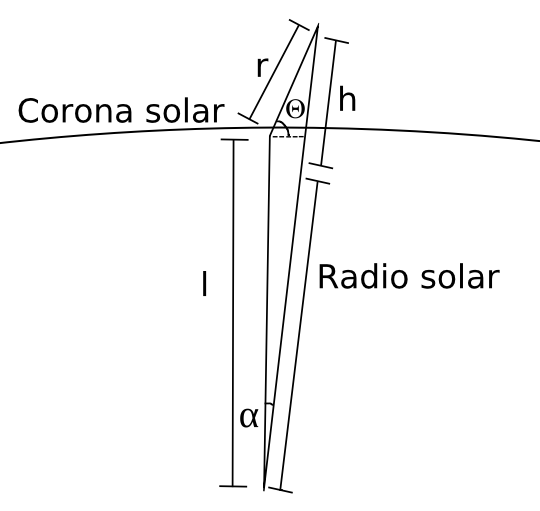
\includegraphics[scale=.8]{arco_magnetico_geometria}
\caption{ Representa la geometr\'ia que se utiliza para adaptar los par\'ametros del arco magn\'etico. }
\label{arco_geometria}
\end{figure}

\begin{figure}[h]
\centering
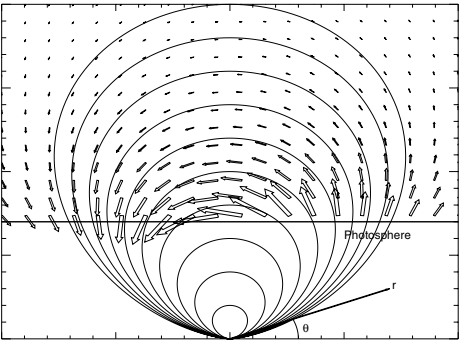
\includegraphics[scale=.8]{magnetic_loop}
\caption{ Imagen tomada del Aswanden. Representa el modelo de arco magn\'etico, donde la longitud de las flechas indican la intensidad del campo, y la direcci\'on en la que apuntan corresponde a la del campo. }
\label{arco_magnetico}
\end{figure}
\clearpage

\subsection{Flujo Emergente}

\textbf{Escala de altura (h). }Es un valor emp\'irico que permite determinar qu\'e tanto se difumina el campo magn\'etico con respecto a la altura. Su valor fue seleccionado de tal forma que los rangos de sus valores caigan dentro de los emp\'iricos que han sido observados. Concretamente, el rango de observaciones emp\'iricas va de 500 a 1000G \citep{VAULT} y para realizar la prueba se tom\'o aleatoriamente el de valor de 200.

\textbf{Flujo magn\'etico (phi). }Representa el campo magn\'etico total que pasa por un \'area determinada. Para realizar las pruebas a la extensi\'on computacional propuesta, se tom\'o como valor del flujo magn\'etico $\phi=2.8x10^{18}$Mx. Si bien existe debate sobre las aproximaciones m\'as precisas con respecto a este valor \citep{magneticflux}; se consider\'o \'este debido a que los resultados del radio inicial del tubo de flujo del modelo de Flujo Emergente fueron coherentes con la teor\'ia (366km \citep{magneticflux} y \citep{VAULT}) al utilizarlo.

\textbf{Intensidad de campo inicial en su base (B0). }Se refiere al valor que toma el campo magn\'etico en la base de su nacimiento, o desde el punto donde se desea comenzar a medir. Los c\'alculos fueron generados considerando distintos valores de campo magn\'etico (0, 500, 1000 y 1500 Gauss), dado que en la literatura se ha dado este valor entre 1000 y 1500 Gauss. La fuerza de la red cromosf\'erica es 1 kG a z=0 con una altura de 500km de acuerdo a Judge (2006 CORREGIR).

\clearpage
\section{Resultados}

En esta secci\'on se presentar\'an los resultados obtenidos de las simulaciones seg\'un los modelos de arcos magn\'eticos y flujo emergente.

\subsection{Micro arco magnetico}
El modelo de arcos magn\'eticos es uno de los modelos m\'as simples y m\'as irreales para simular el comportamineto solar. Sin embargo, a su vez, es un modelo que facilita la comprensi\'on y vizualicaci\'on de la morfolog\'ia del campo magn\'etico de una manera pedag\'ogica.

Los primeros resultados que se presentan, son aquellos concernientes a las pruebas de la codificaci\'on del modelo de arcos magn\'eticos para obtener lo perfiles de los propios arcos magn\'eticos. Particularmente, se realizaron pruebas en los campos magn\'eticos iniciales de 0, 25, 183 y 570G. Con estos valores se obtuvo un perfil del campo magn\'etico a lo largo de la altura; cuyos resultados se pueden apreciar en la Figura \ref{am_Campo_Magnetico}. Como se puede observar, los valores de los campos magn\'eticos arriba de los 1,000 km terminan siendo relativamente peque\~nos, independientemente del valor de entrada. Lo anterior va acorde a la teor\'ia del campo magn\'etico de la crom\'osfera.

Una vez obtenidos los perfiles de los arcos magn\'eticos, ya se puede ajustar la presi\'on de la crom\'osfera a diferentes alturas. Los resultados obtenidos a trav\'es de la extensi\'on al c\'odigo Pakal se representan en la Figura \ref{am_Presion}. En ella se puede ver que conforme m\'as grande es el campo magn\'etico, la presi\'on decrementa menos, manteni\'endose a un valor m\'as alto. 

Despu\'es de obtener los resultado de la presi\'on de la crom\'osfera, se pueden calcular los valores de la densidad del hidr\'ogeno presente en la crom\'osfera. Estos resultados se pueden apreciar en el gr\'afico \ref{am_perfil_de_densidades}. Como se puede observar el comporamiento general es que a mayor campo magn\'etico menor es el gradiente de la densidad. En adici\'on a estos resultados, se muestran tambi\'en dos comparativos entre los resultados de las densidades para diferentes campos magn\'eticos. Estos \'ultimos resultantes se grafican en la Figura \ref{am_diferencias_absolutas} y en la Figura \ref{am_diferencias_relativas}.

\newpage
\begin{figure}[h]
\centering
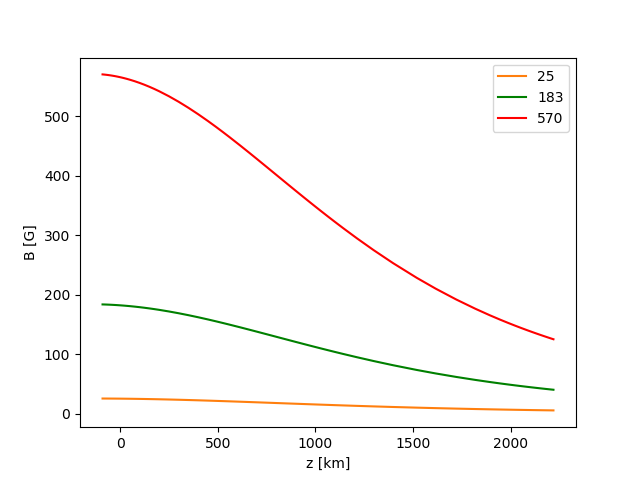
\includegraphics[scale=1]{am_Campo_Magnetico}
\caption{ En esta gr\'afica se describe el comportamiento de la intensidad del campo magn\'etico. }
\label{am_Campo_Magnetico}
\end{figure}


\begin{figure}[h]
\centering
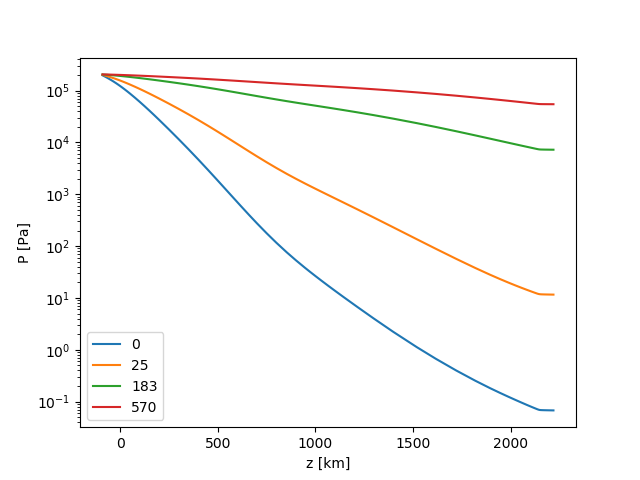
\includegraphics[scale=1]{am_Presion}
\caption{ Aqu\'i se presentan cada una de las salidas de las simulaciones con los distintos valores de campo magn\'etico seg\'un los resultados anteriores.}
\label{am_Presion}
\end{figure}

\begin{figure}[h]
\centering
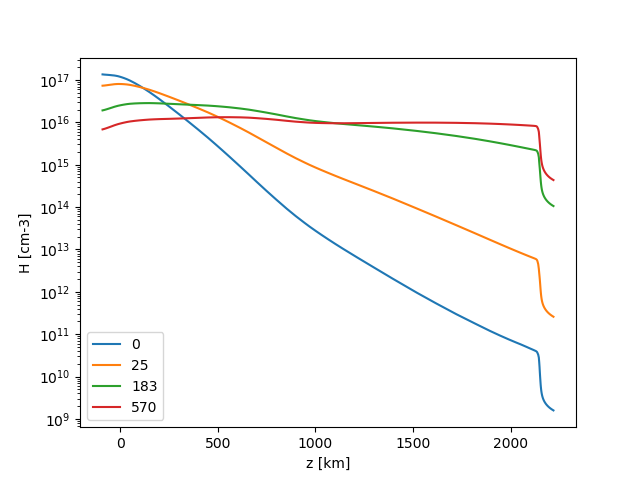
\includegraphics[scale=1]{am_perfil_de_densidades}
\caption{ En esta figura se grafican el perfil de densidades de hidr\'ogeno.}
\label{am_perfil_de_densidades}
\end{figure}

\begin{figure}[h]
\centering
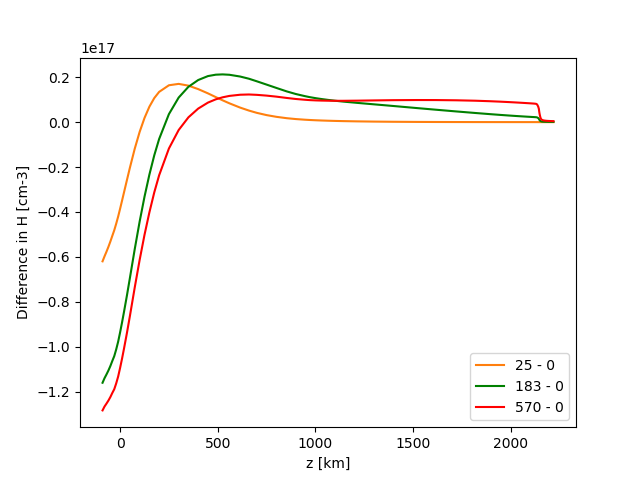
\includegraphics[scale=1]{am_diferencias_absolutas}
\caption{ Aqu\'i se muestra una comparaci\'on entre las diferentes salidas de las densidades del programa.}
\label{am_diferencias_absolutas}
\end{figure}

\begin{figure}[h]
\centering
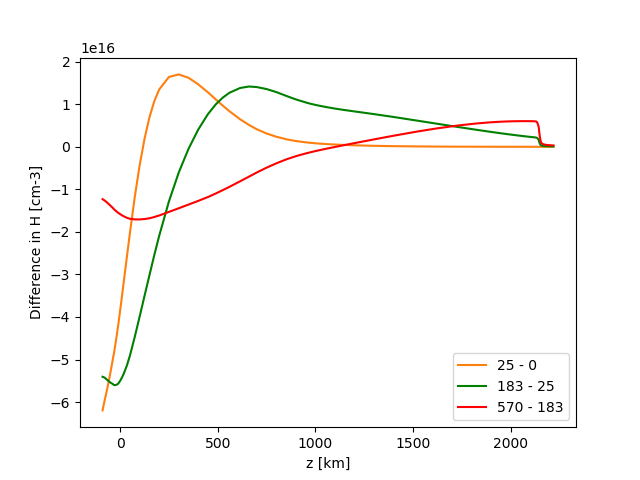
\includegraphics[scale=1]{am_diferencias_relativas}
\caption{ Aqu\'i se muestra un diferencial de cada uno de las salidas de las simulaciones contra las salidas de la simulaci\'on con un valor m\'as bajo.}
\label{am_diferencias_relativas}
\end{figure}


\clearpage
\subsection{Flujo emergente}
El m\'odelo de Flujo emergente es m\'as complejo que el modelo de arcos magn\'eticos, lo que lo hace f\'isicamente m\'as plausible. Sin embargo, es un modelo que no provee de explanantes a la generaci\'on de los campos magn\'eticos.

Al igual que con el modelo anterior. Primero se calcul\'o el perfil de los campos magn\'eticos seg\'un esta teor\'ia. Para esto, y como se explic\'o en secciones anteriores, se utilizaron los valores de 500, 1000 y 1500G. Como se puede apreciar en la Figura \ref{fe_Campo_Magnetico}, la intensidad del campo magn\'etico decae mucho m\'as r\'apido en comparaci\'on con el modelo anterior, a tal grado que para los 1,000km ya es pr\'acticamente despreciable su valor. Este fen\'omeno es a\'un m\'as acertado a las teor\'ias pertinentes.

Similarmente a lo realizado en el modelo de Flujo emergente, una vez obtenidos los valores del perfil de los campos magn\'eticos se procedi\'o a calcular la presi\'on cromosf\'erica. En este modelo se puede entrever un desplazamiento en la ca\'ida de la presi\'on de la crom\'osfera (V\'ease Figura \ref{fe_Presion}). A su vez, con este nuevo valor, se obtuvo el perfil de densidad, el cual presenta un desplazamiento en el gr\'afico para cada valor de campo. 
Finalmente, una vez obtenidos todos estos resultados, tambi\'en se procedi\'o a realizar dos comparativos entre los resultados de las diferentes perfiles de densidades. Los resultados de estas comparativas se pueden apreciar en la Figura \ref{fe_diferencias_absolutas} y Figura \ref{fe_diferencias_relativas}.

\begin{figure}[h]
\centering
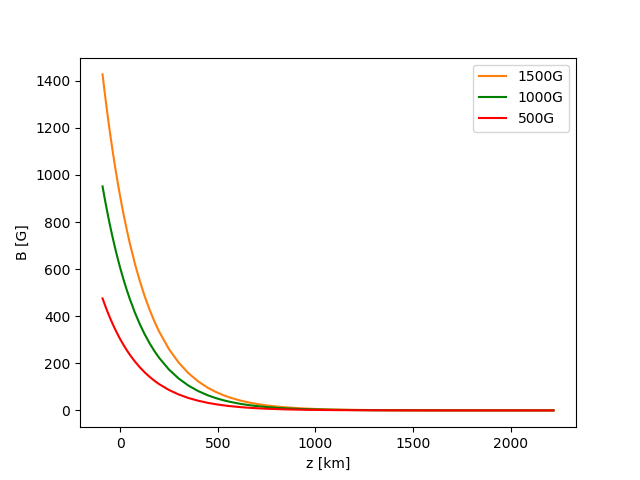
\includegraphics[scale=1]{fe_Campo_Magnetico}
\caption{ En esta gr\'afica se describe el comportamiento de la intensidad del campo magn\'etico. }
\label{fe_Campo_Magnetico}
\end{figure}

\begin{figure}[h]
\centering
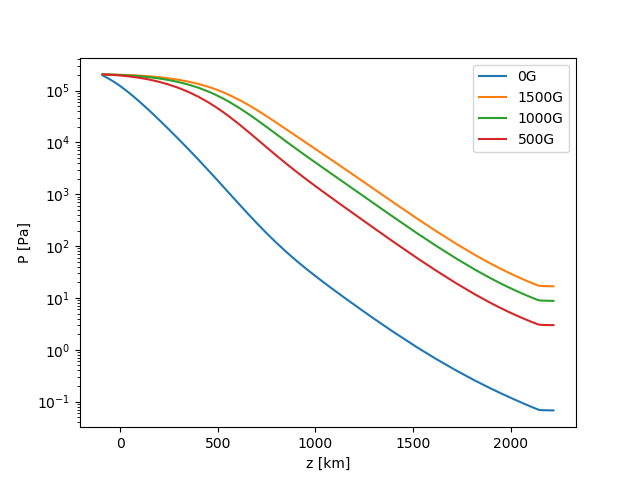
\includegraphics[scale=1]{fe_Presion}
\caption{ Aqu\'i se presentan cada una de las salidas de las simulaciones con los distintos valores de campo magn\'etico seg\'un los resultados anteriores.}
\end{figure}

\begin{figure}[h]
\centering
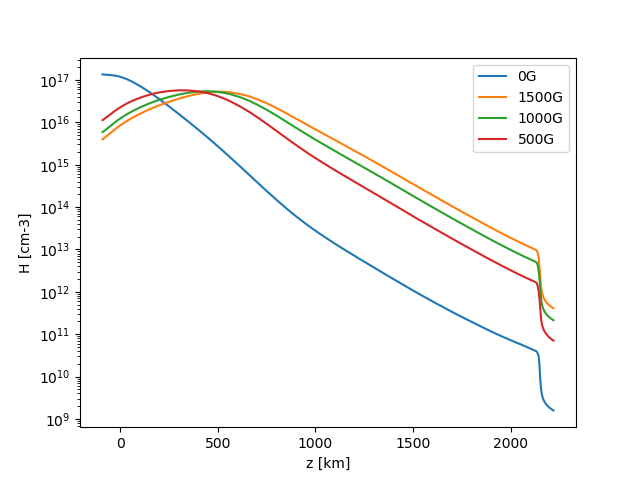
\includegraphics[scale=1]{fe_perfil_de_densidades}
\caption{ En esta figura se grafican el perfil de densidades de hidr\'ogeno.}
\label{fe_perfil_de_densidades}
\end{figure}


\begin{figure}[h]
\centering
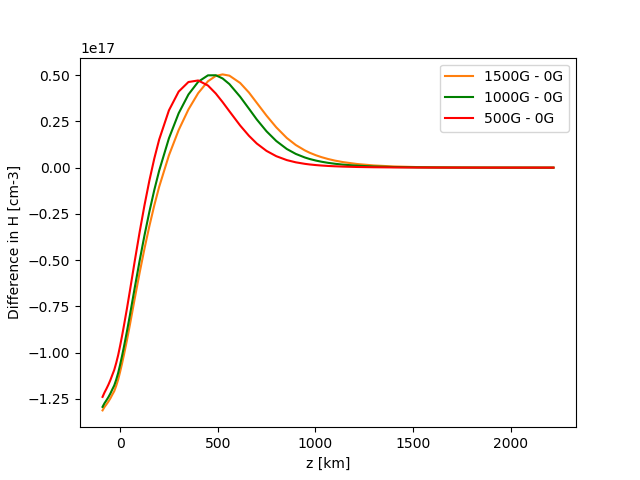
\includegraphics[scale=1]{fe_diferencias_absolutas}
\caption{ Aqu\'i se muestra una comparaci\'on entre las diferentes salidas de las densidades del programa.}
\label{fe_diferencias_absolutas}
\end{figure}

\begin{figure}[h]
\centering
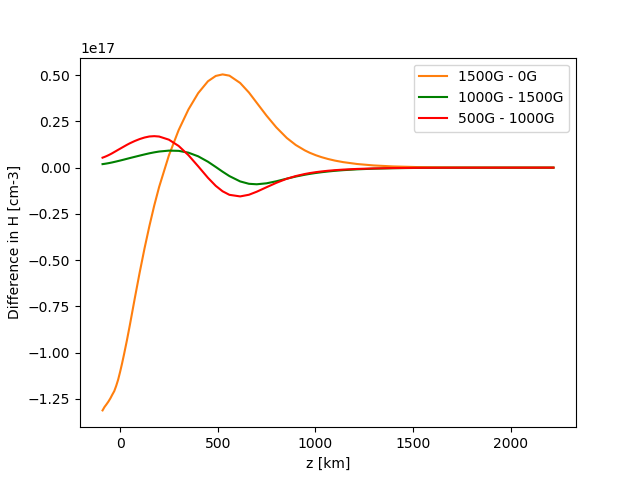
\includegraphics[scale=1]{fe_diferencias_relativas}
\caption{ Aqu\'i se muestra un diferencial de cada uno de las salidas de las simulaciones contra las salidas de la simulaci\'on con un valor m\'as bajo.}
\label{fe_diferencias_relativas}
\end{figure}
\clearpage

\chapter{Discusi\'on y conclusiones}
Comparaci\'on entre ambos modelos, discusion y resultados

aproximaci\'on te\'orica

\chapter{Anexos}

\begin{figure}[h]
\centering
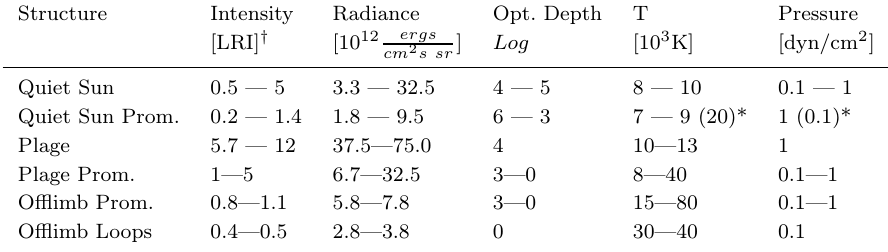
\includegraphics[scale=.7]{tabla_flares}
\caption{ Diagn\'ostico cualitativo del plasma para varios tipos de estructuras.\newline
*Es posible que tengan espesor \'optico reducido. \newline
$^+$Ly$\alpha$ intensidad relativa (LRI). LRI = 1 representa la media de la regi\'on de Sol Quieto.}
\label{tabla_flares}
\end{figure}


\nocite{*}

\newpage
\printbibliography

\end{document}
